%  A simple AAU report template.
%  2015-05-08 v. 1.2.0
%  Copyright 2010-2015 by Jesper Kjær Nielsen <jkn@es.aau.dk>
%
%  This is free software: you can redistribute it and/or modify
%  it under the terms of the GNU General Public License as published by
%  the Free Software Foundation, either version 3 of the License, or
%  (at your option) any later version.
%
%  This is distributed in the hope that it will be useful,
%  but WITHOUT ANY WARRANTY; without even the implied warranty of
%  MERCHANTABILITY or FITNESS FOR A PARTICULAR PURPOSE.  See the
%  GNU General Public License for more details.
%
%  You can find the GNU General Public License at <http://www.gnu.org/licenses/>.
%
%  A simple AAU report template.
%  2015-05-08 v. 1.2.0
%  Copyright 2010-2015 by Jesper Kjær Nielsen <jkn@es.aau.dk>
%
%  This is free software: you can redistribute it and/or modify
%  it under the terms of the GNU General Public License as published by
%  the Free Software Foundation, either version 3 of the License, or
%  (at your option) any later version.
%
%  This is distributed in the hope that it will be useful,
%  but WITHOUT ANY WARRANTY; without even the implied warranty of
%  MERCHANTABILITY or FITNESS FOR A PARTICULAR PURPOSE.  See the
%  GNU General Public License for more details.
%
%  You can find the GNU General Public License at <http://www.gnu.org/licenses/>.
%
\documentclass[11pt,a4paper]{report}
%%%%%%%%%%%%%%%%%%%%%%%%%%%%%%%%%%%%%%%%%%%%%%%%
% Language, Encoding and Fonts
% http://en.wikibooks.org/wiki/LaTeX/Internationalization
%%%%%%%%%%%%%%%%%%%%%%%%%%%%%%%%%%%%%%%%%%%%%%%%
% Select encoding of your inputs. Depends on
% your operating system and its default input
% encoding. Typically, you should use
%   Linux  : utf8 (most modern Linux distributions)
%            latin1 
%   Windows: ansinew
%            latin1 (works in most cases)
%   Mac    : applemac
% Notice that you can manually change the input
% encoding of your files by selecting "save as"
% an select the desired input encoding. 
\usepackage[utf8]{inputenc}
% Make latex understand and use the typographic
% rules of the language used in the document.
\usepackage[danish,english]{babel}
% Use the palatino font
\usepackage[sc]{mathpazo}
\linespread{1.05}         % Palatino needs more leading (space between lines)
% Choose the font encoding
\usepackage[T1]{fontenc}
%%%%%%%%%%%%%%%%%%%%%%%%%%%%%%%%%%%%%%%%%%%%%%%%
% Graphics and Tables
% http://en.wikibooks.org/wiki/LaTeX/Importing_Graphics
% http://en.wikibooks.org/wiki/LaTeX/Tables
% http://en.wikibooks.org/wiki/LaTeX/Colors
%%%%%%%%%%%%%%%%%%%%%%%%%%%%%%%%%%%%%%%%%%%%%%%%
% load a colour package
\usepackage{xcolor}
\definecolor{aaublue}{RGB}{33,26,82}% dark blue
% The standard graphics inclusion package
\usepackage{graphicx}
% Set up how figure and table captions are displayed
\usepackage{caption}
\captionsetup{%
  font=footnotesize,% set font size to footnotesize
  labelfont=bf % bold label (e.g., Figure 3.2) font
}
% Make the standard latex tables look so much better
\usepackage{array,booktabs}
% Enable the use of frames around, e.g., theorems
% The framed package is used in the example environment
\usepackage{framed}

%%%%%%%%%%%%%%%%%%%%%%%%%%%%%%%%%%%%%%%%%%%%%%%%
% Mathematics
% http://en.wikibooks.org/wiki/LaTeX/Mathematics
%%%%%%%%%%%%%%%%%%%%%%%%%%%%%%%%%%%%%%%%%%%%%%%%
% Defines new environments such as equation,
% align and split 
\usepackage{amsmath}
% Adds new math symbols
\usepackage{amssymb}
% Use theorems in your document
% The ntheorem package is also used for the example environment
% When using thmmarks, amsmath must be an option as well. Otherwise \eqref doesn't work anymore.
\usepackage[framed,amsmath,thmmarks]{ntheorem}

%%%%%%%%%%%%%%%%%%%%%%%%%%%%%%%%%%%%%%%%%%%%%%%%
% Page Layout
% http://en.wikibooks.org/wiki/LaTeX/Page_Layout
%%%%%%%%%%%%%%%%%%%%%%%%%%%%%%%%%%%%%%%%%%%%%%%%
% Change margins, papersize, etc of the document
\usepackage[
  inner=28mm,% left margin on an odd page
  outer=41mm,% right margin on an odd page
  ]{geometry}
% Modify how \chapter, \section, etc. look
% The titlesec package is very configureable
\usepackage{titlesec}
\titleformat{\chapter}[display]{\normalfont\huge\bfseries}{\chaptertitlename\ \thechapter}{20pt}{\Huge}
\titleformat*{\section}{\normalfont\Large\bfseries}
\titleformat*{\subsection}{\normalfont\large\bfseries}
\titleformat*{\subsubsection}{\normalfont\normalsize\bfseries}
%\titleformat*{\paragraph}{\normalfont\normalsize\bfseries}
%\titleformat*{\subparagraph}{\normalfont\normalsize\bfseries}

% Clear empty pages between chapters
\let\origdoublepage\cleardoublepage
\newcommand{\clearemptydoublepage}{%
  \clearpage
  {\pagestyle{empty}\origdoublepage}%
}
\let\cleardoublepage\clearemptydoublepage

% Change the headers and footers
\usepackage{fancyhdr}
\pagestyle{fancy}
\fancyhf{} %delete everything
\renewcommand{\headrulewidth}{0pt} %remove the horizontal line in the header

\fancyhead[L]{\small\nouppercase\rightmark} %uneven page - section title
\fancyhead[R]{\thepage} %page number on all pages
% Do not stretch the content of a page. Instead,
% insert white space at the bottom of the page
\raggedbottom
% Enable arithmetics with length. Useful when
% typesetting the layout.
\usepackage{calc}

%%%%%%%%%%%%%%%%%%%%%%%%%%%%%%%%%%%%%%%%%%%%%%%%
% Bibliography
% http://en.wikibooks.org/wiki/LaTeX/Bibliography_Management
%%%%%%%%%%%%%%%%%%%%%%%%%%%%%%%%%%%%%%%%%%%%%%%%
\usepackage[backend=bibtex,
  bibencoding=utf8
  ]{biblatex}
\addbibresource{bib/mybib}

%%%%%%%%%%%%%%%%%%%%%%%%%%%%%%%%%%%%%%%%%%%%%%%%
% Misc
%%%%%%%%%%%%%%%%%%%%%%%%%%%%%%%%%%%%%%%%%%%%%%%%
% Add bibliography and index to the table of
% contents
\usepackage[nottoc]{tocbibind}
\usepackage{csquotes}
% Add the command \pageref{LastPage} which refers to the
% page number of the last page
\usepackage{lastpage}
% Add todo notes in the margin of the document
\usepackage[
%  disable, %turn off todonotes
  colorinlistoftodos, %enable a coloured square in the list of todos
  textwidth=\marginparwidth, %set the width of the todonotes
  textsize=scriptsize, %size of the text in the todonotes
  ]{todonotes}
  
\usepackage{float}
\usepackage{tabu}
\usepackage{array}
\usepackage{longtable}
\usetikzlibrary{fit,shapes}
\restylefloat{table} %

%%%%%%%%%%%%%%%%%%%%%%%%%%%%%%%%%%%%%%%%%%%%%%%%
% Hyperlinks
% http://en.wikibooks.org/wiki/LaTeX/Hyperlinks
%%%%%%%%%%%%%%%%%%%%%%%%%%%%%%%%%%%%%%%%%%%%%%%%
% Enable hyperlinks and insert info into the pdf
% file. Hypperref should be loaded as one of the 
% last packages
\usepackage{hyperref}
\hypersetup{%
	plainpages=false,%
	pdfauthor={Author(s)},%
	pdftitle={Title},%
	pdfsubject={Subject},%
	bookmarksnumbered=true,%
	colorlinks=false,%
	citecolor=black,%
	filecolor=black,%
	linkcolor=black,% you should probably change this to black before printing
	urlcolor=black,%
	pdfstartview=FitH%
}

% code
\usepackage{color}
\usepackage{listings}
\usepackage{inconsolata}
% coding colors defined %
\definecolor{codegreen}{rgb}{0,0.6,0}
\definecolor{codegray}{rgb}{0.2,0.2,0.2}
\definecolor{codeblue}{rgb}{0.13,0.13,1}
\definecolor{codered}{rgb}{0.9,0,0}

 
\lstset{
  basicstyle=\tiny,        % the size of the fonts that are used for the code
  language=Java,
  showspaces=false,
  showtabs=false,
  breaklines=true,
  showstringspaces=false,
  breakatwhitespace=true,
  frame=single,
  commentstyle=\color{codered},
  keywordstyle=\color{codeblue},
  stringstyle=\color{codegreen},
  identifierstyle=\color{codegray},
  numbers=left,
  numbersep=5pt,
  numberstyle=\footnotesize\color{codered},
  emph={node,out,builder,errorHandler,messageList,sb,type,symtable,Id,ID},
  emphstyle={\color{codeblue}},
  basicstyle=\ttfamily,
  moredelim=[il][\textcolor{orange}]{$$},
  moredelim=[is][\textcolor{orange}]{\%\%}{\%\%}
}% package inclusion and set up of the document
% see, e.g., http://en.wikibooks.org/wiki/LaTeX/Formatting#Hyphenation
% for more information on word hyphenation
\hyphenation{ex-am-ple hy-phen-a-tion short}
\hyphenation{long la-tex}% 
%  A simple AAU report template.
%  2015-05-08 v. 1.2.0
%  Copyright 2010-2015 by Jesper Kjær Nielsen <jkn@es.aau.dk>
%
%  This is free software: you can redistribute it and/or modify
%  it under the terms of the GNU General Public License as published by
%  the Free Software Foundation, either version 3 of the License, or
%  (at your option) any later version.
%
%  This is distributed in the hope that it will be useful,
%  but WITHOUT ANY WARRANTY; without even the implied warranty of
%  MERCHANTABILITY or FITNESS FOR A PARTICULAR PURPOSE.  See the
%  GNU General Public License for more details.
%
%  You can find the GNU General Public License at <http://www.gnu.org/licenses/>.
%
%
%
% see, e.g., http://en.wikibooks.org/wiki/LaTeX/Customizing_LaTeX#New_commands
% for more information on how to create macros

%%%%%%%%%%%%%%%%%%%%%%%%%%%%%%%%%%%%%%%%%%%%%%%%
% Macros for the titlepage
%%%%%%%%%%%%%%%%%%%%%%%%%%%%%%%%%%%%%%%%%%%%%%%%
%Creates the aau titlepage
\newcommand{\aautitlepage}[3]{%
  {
    %set up various length
    \ifx\titlepageleftcolumnwidth\undefined
      \newlength{\titlepageleftcolumnwidth}
      \newlength{\titlepagerightcolumnwidth}
    \fi
    \setlength{\titlepageleftcolumnwidth}{0.5\textwidth-\tabcolsep}
    \setlength{\titlepagerightcolumnwidth}{\textwidth-2\tabcolsep-\titlepageleftcolumnwidth}
    %create title page
    \thispagestyle{empty}
    \noindent%
    \begin{tabular}{@{}ll@{}}
      \parbox{\titlepageleftcolumnwidth}{
        \iflanguage{danish}{%
          
\includegraphics[width=\titlepageleftcolumnwidth]{figures/aau_logo_da}
        }{%
          
\includegraphics[width=\titlepageleftcolumnwidth]{figures/aau_logo_en}
        }
      } &
      \parbox{\titlepagerightcolumnwidth}{\raggedleft\sf\small
        #2
      }\bigskip\\
       #1 &
      \parbox[t]{\titlepagerightcolumnwidth}{%
      \textbf{Abstract:}\bigskip\par
        \fbox{\parbox{\titlepagerightcolumnwidth-2\fboxsep-2\fboxrule}{%
          #3
        }}
      }\\
    \end{tabular}
    \vfill
    \iflanguage{danish}{%
      \noindent{\footnotesize\emph{Rapportens indhold er frit tilgængeligt, men offentliggørelse (med kildeangivelse) må kun ske efter aftale med forfatterne.}}
    }{%
      \noindent{\footnotesize\emph{The content of this report is freely available, but publication (with reference) may only be pursued due to agreement with the author.}}
    }
    \clearpage
  }
}

%Create english project info
\newcommand{\englishprojectinfo}[8]{%
  \parbox[t]{\titlepageleftcolumnwidth}{
    \textbf{Title:}\\ #1\bigskip\par
    \textbf{Theme:}\\ #2\bigskip\par
    \textbf{Project Period:}\\ #3\bigskip\par
    \textbf{Project Group:}\\ #4\bigskip\par
    \textbf{Participant(s):}\\ #5\bigskip\par
    \textbf{Supervisor(s):}\\ #6\bigskip\par
    \textbf{Copies:} #7\bigskip\par
    \textbf{Page Numbers:} \pageref{LastPage}\bigskip\par
    \textbf{Date of Completion:}\\ #8
  }
}

%Create danish project info
\newcommand{\danishprojectinfo}[8]{%
  \parbox[t]{\titlepageleftcolumnwidth}{
    \textbf{Titel:}\\ #1\bigskip\par
    \textbf{Tema:}\\ #2\bigskip\par
    \textbf{Projektperiode:}\\ #3\bigskip\par
    \textbf{Projektgruppe:}\\ #4\bigskip\par
    \textbf{Deltager(e):}\\ #5\bigskip\par
    \textbf{Vejleder(e):}\\ #6\bigskip\par
    \textbf{Oplagstal:} #7\bigskip\par
    \textbf{Sidetal:} \pageref{LastPage}\bigskip\par
    \textbf{Afleveringsdato:}\\ #8
  }
}

%%%%%%%%%%%%%%%%%%%%%%%%%%%%%%%%%%%%%%%%%%%%%%%%
% An example environment
%%%%%%%%%%%%%%%%%%%%%%%%%%%%%%%%%%%%%%%%%%%%%%%%
\theoremheaderfont{\normalfont\bfseries}
\theorembodyfont{\normalfont}
\theoremstyle{break}
\def\theoremframecommand{{\color{gray!50}\vrule width 5pt \hspace{5pt}}}
\newshadedtheorem{exa}{Example}[chapter]
\newenvironment{example}[1]{%
		\begin{exa}[#1]
}{%
		\end{exa}
}% my new macros
\usepackage{pdfpages}
\usepackage[T1]{fontenc}
\usepackage{semantic}
\usepackage{url}

\begin{document}
%frontmatter
\pagestyle{empty} %disable headers and footers
\pagenumbering{roman} %use roman page numbering in the frontmatter
%  A simple AAU report template.
%  2015-05-08 v. 1.2.0
%  Copyright 2010-2015 by Jesper Kjær Nielsen <jkn@es.aau.dk>
%
%  This is free software: you can redistribute it and/or modify
%  it under the terms of the GNU General Public License as published by
%  the Free Software Foundation, either version 3 of the License, or
%  (at your option) any later version.
%
%  This is distributed in the hope that it will be useful,
%  but WITHOUT ANY WARRANTY; without even the implied warranty of
%  MERCHANTABILITY or FITNESS FOR A PARTICULAR PURPOSE.  See the
%  GNU General Public License for more details.
%
%  You can find the GNU General Public License at <http://www.gnu.org/licenses/>.
%
\pdfbookmark[0]{Front page}{label:frontpage}%
\begin{titlepage}
  \addtolength{\hoffset}{0.5\evensidemargin-0.5\oddsidemargin} %set equal margins on the frontpage - remove this line if you want default margins
  \noindent%
  \begin{tabular}{@{}p{\textwidth}@{}}
    \toprule[2pt]
    \midrule
    \vspace{0.2cm}
    \begin{center}
    \Huge{\textbf{
      Home Automation% insert your title here
    }}
    \end{center}
    \begin{center}
      \Large{
        - Subtitle -% insert your subtitle here
      }
    \end{center}
    \vspace{0.2cm}\\
    \midrule
    \toprule[2pt]
  \end{tabular}
  \vspace{4 cm}
  \begin{center}
    {\large
      Project Report%Insert document type (e.g., Project Report)
    }\\
    \vspace{0.2cm}
    {\Large
      sw415f19%Insert your group name or real names here
    }
  \end{center}
  \vfill
  \begin{center}
  Aalborg University\\
  Software
  \end{center}
\end{titlepage}
\clearpage
\pdfbookmark[0]{English title page}{label:titlepage_en}
\aautitlepage{%
  \englishprojectinfo{
    Ezuino %title
  }{%
    Programming Language %theme
  }{%
    Spring Semester 2019 %project period
  }{%
    sw415f19 % project group
  }{%
    %list of group members
    Casper Andreas Klein\\ 
    Jonas Bylling Andersen\\
    Laurits Brøcker\\
    Peter Kjær\\
    Peter Minh Do\\
    Samuel Alexander Vall Andersen
  }{%
    %list of supervisors
    Razvan-Gabriel Cirstea
  }{%
    1 % number of printed copies
  }{%
    May 28, 2019 % date of completion
  }%
}{%department and address
  \textbf{Software}\\
  Aalborg University\\
  \href{http://www.aau.dk}{http://www.aau.dk}
}{% the abstract
    This paper seeks to analyze, create, and discuss the features and choices in regards to creating a new programming language, as well as a compiler for said language, for use by novice programmers on arduinos or comparable single-board-computers.
}

\cleardoublepage
% {\selectlanguage{danish}
% \pdfbookmark[0]{Danish title page}{label:titlepage_da}
% \aautitlepage{%
%   \danishprojectinfo{
%     Rapportens titel %title
%   }{%
%     Semestertema %theme
%   }{%
%     Forårssemestret 2019 %project period
%   }{%
%     sw415f19 % project group
%   }{%
%     %list of group members
%     Casper Andreas Klein\\ 
%     Jonas Bylling Andersen\\
%     Laurits Brøcker\\
%     Peter Kjær\\
%     Peter Minh Do\\
%     Samuel Alexander Vall Andersen
%   }{%
%     %list of supervisors
%     Razvan-Gabriel Cirstea
%   }{%
%     1 % number of printed copies
%   }{%
%     28. Maj 2019 % date of completion
%   }%
% }{%department and address
%   \textbf{Software}\\
%   Aalborg Universitet\\
%   \href{http://www.aau.dk}{http://www.aau.dk}
% }{% the abstract
%   Her er resuméet
% }}
\cleardoublepage
\pdfbookmark[0]{Contents}{label:contents}
\pagestyle{fancy} %enable headers and footers again
\tableofcontents
\chapter*{Preface\markboth{Preface}{Preface}}\label{ch:preface}
\addcontentsline{toc}{chapter}{Preface}
Here is the preface. You should put your signatures at the end of the preface.

\vspace{\baselineskip}\hfill Aalborg University, \today
\vfill\noindent
\begin{minipage}[b]{0.45\textwidth}
 \centering
 \rule{\textwidth}{0.5pt}\\
  Casper Andreas Klein\\
 {\footnotesize <cklein17@student.aau.dk>}
\end{minipage}
\hfill
\begin{minipage}[b]{0.45\textwidth}
 \centering
 \rule{\textwidth}{0.5pt}\\
  Jonas Bylling Andersen\\
 {\footnotesize <jban18@student.aau.dk>}
\end{minipage}
\vspace{3\baselineskip}

\vfill\noindent
\begin{minipage}[b]{0.45\textwidth}
 \centering
 \rule{\textwidth}{0.5pt}\\
  Laurits Brøcker\\
 {\footnotesize <lbrack17@student.aau.dk>}
\end{minipage}
\hfill
\begin{minipage}[b]{0.45\textwidth}
 \centering
 \rule{\textwidth}{0.5pt}\\
  Peter Kjær\\
 {\footnotesize <pkjar16@student.aau.dk>}
\end{minipage}
\vspace{3\baselineskip}

\vfill\noindent
\begin{minipage}[b]{0.45\textwidth}
 \centering
 \rule{\textwidth}{0.5pt}\\
  Peter Minh Do\\
 {\footnotesize <pdo17@student.aau.dk>}
\end{minipage}
\hfill
\begin{minipage}[b]{0.45\textwidth}
 \centering
 \rule{\textwidth}{0.5pt}\\
  Samuel Alexander Vall Andersen\\
 {\footnotesize <sava17@student.aau.dk>}
\end{minipage}
\vspace{3\baselineskip}
%mainmatter
\pagenumbering{arabic} %use arabic page numbering in the mainmatter


%struktur af rapporten


\chapter{Introduction}\label{ch:introduction}
With the rise of cheap microprocessors and humans, innovation came an abundance of new small internet connected devices. These devices are what is called the “Internet of Things”. Gadgets, machines and appliances, which are connected to the internet\cite{iot-definition}. A subgroup within the IoT-subject is Home Automation. Home automation is the process for consumers to automate their home. Some examples are garage doors, light bulbs, thermostats, smart locks, outlets and even curtains. In a research paper\cite{home-auto-growth} on the smart home market, it was clear that in 2017, the worldwide customer spending on smart home was \$84 billion and projected to grow to \$155 billion by 2023. For the hometinkers and hobby-hackers, these products were available too. It started with Arduino in 2003, which had hardware that was cheap and easy to program\cite{arduino-history}. It wasn’t until later that the Arduino gained WiFi capabilities. Pairing the internet capabilities with the easy to learn Arduino C programming could be used to program chips and help from the online community and forming new ideas.

In the later years, the Arduino sparked a new flavor of Arduino like microcontrollers with both WiFi and bluetooth capabilities. Some examples of these internet connected microcontrollers are the ESP8266 (2014) and the ESP32 (2016). Both of which are as cheap as the Arduino (sometimes even \$1), available from most of the world in a GPIO pins that resembles the Arduino, with the added benefit of having WiFi and bluetooth connectivity. However, the programming language on these are different. Since Arduino C is so popular, a community effort has been made to add support for the Arduino SDK to these chips. That means that multiple of the IoT devices are supported by the Arduino IDE and can be written in Arduino C, with the proper libraries.

From a business standpoint, many have started making their products IoT-devices, most of which can be controlled directly from your phone. It opened up new possibilities for doing stuff without having to do them manually. Since companies started creating all the IoT-devices, companies like Google and Apple have begun up for integrating with the home automation devices to lure users onto their platform. Google’ Assistant\cite{google-assistant}, Apple’s Home\cite{apple-homekit} and Amazon’s Alexa\cite{amazon-alexa} are currently the major players in this. They all allow the user to control their automated home in a more centralized and streamlined way than having to control each device from their own app. May it simply be lights to turn on (Eg. Ikea Trådfri bulbs), temperature regulation from night to day (ecobee thermostat) to smart connected fridges (Eg. Samsung Family Hub fridges) amongst other things. 
\section{Introduction (EMPTY)}
\section{Targeted group}
\label{targetedGroup}
Before we can work on language design and ideas, we must find a targeted user group and analyze them, such that we can gather ideas and create a language, which resides towards the initial problem statement. \\
\\
The focus group is between 18 to 45 years old people, who has some interest in technology. Since this may be an abstract target group, the experience on how to use the product may be different. As such, a PACT analysis got made to understand the targeted group better. \\
\\
\textbf{People (P)}: The focus group is people of every class who live in a home. This could be anyone, from larger families to people living by themselves. Age is not restrictive but should be focused to be learned by people 18 years or older. The learning experience on how to use technology varies since seniors can have little to no experience on how to use technology.
\\
\textbf{Activities (A)}: The product should be able to automate a difficult task regarding electronics in general homes. For example when it is Summer, if it gets too warm in the house, the product should automatically open the window and close the window again after it has registered the room temperature. The signal would be when the room temperature cold, and when the temperature is warmer than normally. \\
\\
\textbf{Context (C)}: The product is set up within an indoor and outdoor apartment in all types of weather. To use the product at all times of the day requires an Arduino to program the different devices.\\
\\
\textbf{Technologies (T)}: The technology will use Arduino as the hardware and a charger that will keep the Arduino running. The user should be able to access the code, by any electronic device capable of coding, and should be compatible with any device able to connect and run Arduino hardware. \\
\\
Based on this PACT analysis, we now have a firm grasp of how we can expect the users of our programming language to interact with our language.

\section{Programming Paradigm}
\label{programmingparadigm}
To get an understanding of the programming style and paradigm, we must consider the user group. It is essential to create a language, which is both easy to learn and still rich in features to complete its task. Many languages today are designed for a specific problem domain – an example is Lisp which is useful for symbolic data manipulation and having a complex data structure. The programming language C is good for low-level systems programming, as the programmer has a high level of control over system memory, although an assembly-like language would be too challenging and inefficient for a novice programmer to write in.
As the paradigm is quite essential to any given programming language, it is important to consider which paradigm would best suit the needs of our problem domain.\\
\\
From the earlier analysis, the focus of this system was to create a programming system, in which an ordinary user, without any previous programming experience, can use, with a manual and learn. In this case, the focus group is very novice users, who may have touched a little, to no code in their lifetime. Looking at some early programming languages for this user group, we must consider some earlier programming languages, which has been used in educational purposes and have a low learning curve. Some of the early programming languages which have had success were Basic, which is a high-level programming language, which is a part of the programming paradigm Non-structured, and later procedural (which is structured). Another programming language created for the educational purposes in 1967, named Logo. Logo is a programming language, which is in the family with Lisp, and got the programming paradigms: functional, educational, procedural and reflective.\cite{scott2000programming} \\
\\
To bring a typical pattern in the programming languages which got mentioned in this section, all of them got a common factor, that they run on procedural paradigm, which is the opposite of the modern object-orientated paradigm, which is being used by many of the prominent languages today (Java, C\# etc.). Why is it, that object orientated paradigm is not well used for novice users, for educational purposes? - Looking at an article by Jacques Le Normand on Medium.org, Jacques reflects through this question, and the following reflections came up:\cite{tutlisp}\cite{medlisp} \\
\begin{itemize}
 \item Object orientated paradigm was not the first paradigm, and at most time is not even an appropriate paradigm for smaller tasks however, it is one of the more prevalent paradigms in many industries today.
 \item Object orientation thinking requires much work and can be referred to as English essays, which most students do not particularly enjoy learning to write.\cite{tutlisp}\cite{medlisp}
\end{itemize}
Reflecting through this, object orientated paradigms might not be a good first language, as it got a more profound learning curve than a procedural paradigm. As Jacques mentioned in his article, object orientation requires skills to understand, where procedural programming is straight forward without requiring no knowledge of classes and objects.\\
\\
\section{Arduino}
The target group are users requiring a simple programming language for home automation as determined in \ref{targetedGroup}. As previously concluded in chapter \ref{programmingparadigm}, the programming language should also be procedural to better accommodate users with less experience in programming.
A programming language that fits the need for being procedural and is suited to implement software to physical devices like home automation is the Arduino programming language. Arduino is an open-source electronics platform based on easy-to-use hardware and software. Arduino uses boards that are able to read inputs - light on a sensor, a finger on a button, or a Twitter message - and turn it into an output - activating a motor, turning on an LED. Boards can be controlled by sending a set of instructions to the microcontroller on the board with the Arduino programming language. The Arduino programming language is a dialect of features from the programming languages C which is a procedural imperative, C++, and Arduino Software (IDE)\cite{audionocc}. \\

%The Arduino software is according to themselves, “easy-to-use for beginners, yet flexible enough for advanced users”. It runs on Mac, Windows, and Linux.

Another merit of creating a specialized version of the Arduino programming language is that the software is published as open source, and according to their official website, is available for extension by experienced programmers\cite{audionocc}.

%The environment also is written in Java and based on processing and other open-source software.
%The language can be expanded through C++ libraries and runs on Windows, Mac OS X, and Linux.








\section{Problem scoping}
%This section will describe which features we will not prioritize due to time limitations.\\
%We will not prioritize list and structs. These data type are more complex than the other features to implement and while we do want to include both data types as we think they both serve important purposes we will only implement them if we have sufficient extra time.
%We will not prioritize other control structures than the while loop. As mentioned previously the while loop enables everything the other control structures does and therefore the while loop will be prioritized.

%\subsubsection{Scope of features}
%As there are a lot of IoT devices and other Arduino models, the project will be limited to be developed and tested on Arduino Uno.

%\subsubsection{Scope of tests}
%As it is essential that the compiler does not contain errors, testing will get focused to a greater extent of this project. Testing of the program, JUnit test should be done in the significant fields of code and functionality, together with running automated Continuous Integration (CI), which will run the tests in every build, together with a PR/Code Quality manager running as a static code analyser. Further testing, such as code coverage test, will not be considered in this development phase. \\


%As the scoping reach an end, we can start putting a problem definition together, where we can define the exact problem that we in which can solve with this programming language.

%--------------------------- Old problem 
%This section will be scoping the problem and the product onwards based on the MoSCoW analysis, and the decisions described in this section.  

%he programming language will create a full code generation, which will be mainly focused and limited to Arduino primary programming language, C. The project will only be fully implemented in this language; however, some Java Bytecode generation will be made as well, but not to the full extent. As there is a lot of IoT devices, and other Arduino models, the project will be limited to be developed and tested on an Arduino Uno.  
%Syntax of the programming language will be limited to the analysis part, which will take part in the most common syntax used in programming languages today. The functionality and syntax of the programming language will only be limited to the most crucial parts mentioned in the MoSCoW analysis. All the additional functionality, like Java’s Array List, will not be within this project scope at this time but will be available for further development. 
%As it is essential that the compiler does not contain errors, testing will get focused to a greater extent of this project. Testing of the program, JUnit test should be done in the significant fields of code and functionality, together with running automated Continuous Integration (CI), which will run the tests in every build, together with a PR/Code Quality manager running as a static code analyser. Further testing, such as code coverage test will not get considered in this development phase.  
%As the scoping reach an end, we can start putting a problem definition together, where we can define the exact problem that we in which can solve with this programming language.  



This section will scope down the project, to which priorities are most vital for the project, to be called a success. \\
\\
The goal of the project is to create a programming language, which has the most essential syntax for the language to be use able in all cases. The language will be targeted for usage on an Arduino, and will have the most essential parts of the special syntax, the Arduino uses in its libraries. All the functionality of the Arduino library will not be implemented, as this is not a part of the project frame, and there is way to many special functions and syntax, that it will be scoped down to the most essential parts. \\
\\
The Ezuino programming language will only be code generated for two languages, Arduino C and Java bytecode. The syntax for each of these will be prioritized in a MoSCoW analysis, which will be reviewed in a later chapter. The Ezuino programming language will be made from the most prioritized features first, and going down to the less important features. As the programming language is very big to implement, the project will be scoped to implementing the vital parts at first, leaving some minor syntax priorities to may be discarded if time is critical. \\
\\
In a compiler, it is very important that it does not contain any errors, as it can be frustrating for the users programming their code in the language. As of this, it is vital to have testing, to a greater degree of the compiler. The testing of the project will be mainly focused on the technical part, with using JUnit testing and CI, to avoid any errors in the development process. Other testing will not be included in this project. \\
\\ 
In the problem definition, the goal is to provide a programming language for people, with no or little programming knowledge. To provide a clear acceptance of this problem, multiple user testing should be made for well documenting this problem. In this project, the user testing will be scoped down to 1 user test, as the programming language itself, has the up most priority.


\subsection{MoSCoW}
%-- MoSCoW til language features (Use MoSCoW to clarify the prioritization of the languages features ex. datastructures, if else for etc.)


This section will provide an account of the different elements, which will be prioritized within a MoSCoW analysis. MoSCoW analysis is an abbreviation for Must have, Could Have, Would have and wont have (this time). This analysis will provide an account and ensure that the critical elements in the programming language will be included in the project.

% Please add the following required packages to your document preamble:
% \usepackage{booktabs}

\begin{table}[H]
\begin{tabular}{@{}lll@{}}
\toprule
\caption{Requirements for the programming language}
\textbf{Area}          & \textbf{Subject}        & \textbf{Priority}               \\ \midrule
Data Types             & Integer                 & Must have                       \\
                       & Double                  & Must have                       \\
                       & String                  & Must have                       \\
                       & Boolean                 & Must have                       \\ 
                       & List                    & Must have                     \\
                       & Struct                  & Could have                      \\\midrule
Arithmetic operators   & Addition                & Must have                       \\
                       & Subtraction and negate  & Must have                       \\
                       & Multiplication          & Must have                       \\
                       & Division                & Must have                       \\ \midrule
Logical Operators      & AND                     & Must have                     \\
                       & OR                      & Must have                     \\ 
                       & NOT                     & Must have                     \\\midrule
Relational Operators   & Equal                   & Must have                       \\
                       & Not equal               & Must have                       \\
                       & Less than               & Must have                       \\
                       & Less than or equal      & Must have                       \\
                       & Greater than            & Must have                       \\
                       & Greater than or equal   & Must have                       \\ \midrule
Assignment operators   & Assignment              & Must have                       \\
                       & Assignment with 
                         arithmetic operations   & Wont have (this time)          \\ \midrule
Control Structures     & If                      & Must have                       \\
                       & Else                    & Must have                       \\
                       & While                   & Must have                       \\\midrule
%                       & For                     & Wont have (this time)           \\\midrule
Functions and program structure     & Function declarations             & Must have \\
                                    & Function calls                    & Must have \\ 
                                    & Arduino basic functions           & Must have \\ 
                                    & Other Arduino library functions   & Could have \\
                                    & Setup and Loop                    & Must have \\ \midrule
Casting and parsing                 & Casting to string and other data types         & Must have \\
                                    & Parsing from string to other data types        & Could have \\ \midrule
                       
\end{tabular}
\end{table}

\iffalse 
This is commented out for saving purpose
\subsection{Must have}
\textbf{Data Types} 

\begin{itemize} 
    \item Integer
    \item Double
    \item String
    \item Boolean
\end{itemize} 
\\
\textbf{Binary Operators} \\
\begin{itemize} 
    \item Addictive
    \item Multiplicative
    \item Division
    \item Plus
    \item Minus
    \item Less
    \item LessThanOrEqual
    \item Greater
    \item GreaterThanOrEqual
\end{itemize} 
\\
\textbf{Unary Operators} \\
\begin{itemize} 
    \item Not
    \item Minus
\end{itemize}
\\
\textbf{Control Structures} \\
\begin{itemize} 
    \item If
    \item Else
    \item While
    \item Return
\end{itemize} 
\\
\subsection{Should have }
\textbf{Data Types }
\begin{itemize} 
    \item Booleans
\end{itemize} 
\\
\textbf{Binary Operators} 
\begin{itemize} 
    \item And
    \item Or
\end{itemize} 
\\
\textbf{Homogeneous Collection }
\begin{itemize} 
    \item List
\end{itemize} 
\\
\subsection{Could have}
\textbf{Data Types }
\begin{itemize} 
    \item Char
\end{itemize} 
\\
\subsection{Would have but not at this time }
\\
\textbf{Data Types }
\begin{itemize} 
    \item Floats
    \item Unsigned Numbers
\end{itemize} 
\\
\textbf{Bitwise Operators }
\begin{itemize} 
    \item All bitwise shifts and operations. 
\end{itemize} 

\fi

\section{Problem definition}
 After gathering information about current solutions and explaining how the syntax and statement works from the initial problem, is to define the problem that this project is trying to solve. \\ The objective in this project is to create a programming language that is easy to use for an average user who may or may not have any experience in programming, while the programming language will be implemented to an Arduino device that will automate a device at home, which is called home automation. So the problem definition is formulated as:\\
\\
\textit{It is a problem that users sometimes forget to close their windows or turn off their lamps, which will increase their bill in electricity, therefore is it possible to create a programming language connected to a device to make those forgetful task automatically?}




\chapter{Language Design}\label{ch:langspec}
\section{Language Design Criteria and Language Features}
The goal of Ezuino is to be an easier option for people previously unfamiliar with code. To evaluate whether this criteria has been achieved or not, it is necessary to have metrics to evaluate the language. We have chosen the metrics from \cite{conceptsOfProgrammingLanguages}, that evaluates a language based on the metrics readability, writability and orthogonality and cost. For the purpose of a language meant for home automation for people new to programming, and not a programming language meant for industry, the metric cost will not be taken into account. \\
After describing the theory behind the evaluation criteria, the language features Ezuino will include compared to Arduino C will be described. How these features affect language design criteria will also be covered. At the end of the chapter there will be an summary of all the features that are affected by the language design criteria.
\subsection{Language Design Criteria}
\label{language-design-criteria}
\label{design-criteria-theory}
\subsection*{Readability}
\subsubsection*{Overall Simplicity}
Overall simplicity of a programming language is affected by the amount of basic structures, similarity between previous learned languages, feature multiplicity, operator overloading and trade-off between high and low level languages.
It is easier to learn a language with fewer basic constructs than one with a larger amount. Programmers that use large languages usually do not learn all its features. \\\
Readability problems can occur when the same syntax have different meaning than the one the reader is familiar with.  \\\
Feature multiplicity is when there are multiple ways to accomplish the same operation increasing possible complexity. \\
Operator overloading happens when operators can have multiple uses depending on the context. An example of an commonly accepted operator overloading is using + for both integer- and floating point addition. \\
Simplicity in readability also has an trade-off in terms of comparing high to low level languages. An high level language with more complex control statements might make an language easier to read, i.e. assembly compared to Java.

\subsection*{Orthogonality}
"Orthogonality in a programming language means that a relatively small set
of primitive constructs can be combined in a relatively small number of ways
to build the control and data structures of the language. Furthermore, every possible combination of primitives is legal and meaningful."
Bad orthogonality is when a programmer can use constructs in combinations where the result is not obvious. An example of this is "+" in C allows the addition of characters and integers. As it does not give a compiler error it can take longer to find the error as well.
An limited amount of combinations and therefore orthogonality increases the overall simplicity of an language.

\subsubsection*{Data Types}
An adequate amount of data types to fit the need of different situations significantly increases readability . For example, in a languages without the boolean datatype a statement 
isReady = 1 would signal true. Where in a language with boolean isReady = true would be the equivalent, which is more clear.

\subsubsection*{Syntax Design}
\begin{itemize}
    \item Simplicity versus readability in compound statements. Fontran 95 and Ada, uses end if and end loop to differentiate between when an if statement and loop ends, instead of using curly brackets for both like they do in C and Java.
    \item Allowing keywords to also be legal variable names can be confusing and decrease readability.
\end{itemize}

\subsection*{Writability}
Writability is measured in how easily a language can be used to create programs within a chosen problem domain. 
A language must be efficient at the field it was designed for, ie. if it was designed for graphical interfaces, that is the domain it must be comparatively efficient.
\subsubsection*{Simplicity and Orthogonality}
Simplicity and orthogonality applies the same for writability as in readability. In writability confusion due to complex orthogonality can also lead to unintended use of features. It can also be harder to detect errors when  nearly any combination of primitives is legal.
\subsubsection*{Expressivity}
An high degree of expressivity is having convenient, rather than cumbersome, ways of specifying computation. Examples of this are powerful ways to execute a great of deal of computations like for loops in a very small program while also counting the iterations. It could also be using the special words "and" and "then" like in Ada for short-circuit evaluation of a Boolean expression.
\subsubsection*{Reliability}
Reliability is closely related to readability and writability. A language has natural ways to support algorithms will use fewer unnatural approaches to solving problems and are more likely to be correct for all possible situations.
Reliability is also affected by a languages implementation of Type checking, Exception handling and Aliasing. 
\subsubsection*{Type Checking}
Type checking is how the language ensures that types are used in a legal way. Java is very reliable in the sense that it has virtually eliminated type errors by type checking all variable and expressions during compile time .
\subsubsection*{Exception handling}
"The ability of a program to intercept run- time errors (as well as other
unusual conditions detectable by the program), take corrective measures, and
then continue is an obvious aid to reliability."
Some languages like C do not feature exception handling, while other languages like C\# and Java does. 
\subsubsection*{Aliasing}
"Loosely defined, aliasing is having two or more distinct names in a program that can be used to access the same memory cell." \\
Allowing aliasing requires the programmer to remember which names are referring to the same memory cell and failure to do this can lead to bugs.  It is now generally accepted
that aliasing is a dangerous feature in a programming language .




%\subsubsection*{Cost}
%The cost of a programming language depend on many characteristics .
%\begin{itemize}
 %   \item The cost of training programmers to use the language. How costly that is depends largely on the simplicity and orthogonality of the language.
 %   \item Writability affect the continues cost of using the programming language, and the cost of using the programming language is also closely related to how well the programming language fit the purpose of the application. 
 %   \item Compiling cost can be a concern depending on who leases the compiler. 
 %   \item The cost of a language is also the execution time of the code it produces. There is typically an trade-off between compilation versus execution time, and which is more important depend on how many times a program is expected to be run after compilation. 
 %   \item The cost in maintainability because of readability. Maintainability is a huge factor in cost. "It has
 %   been estimated that for large software systems with relatively long lifetimes, maintenance costs can be as high as two to four times as much as development costs (Sommerville, 2010)."
 %   \item Cost of poor reliability. In industries where mistakes are very expensive reliability is an important cost when considering a programming language.
%\end{itemize}








\subsection{Language Features}
\label{language-features}
* All content in this section is based on the C programming language book \cite{kernighan1988c}.\\
This section will reflect on the different language features, operators and structures in the Ezuino code. We will go through each group of operator/structure, and discuss each element, compare them which functionality get included in the Ezuino programming language, and excluded from the target language, which is Arduino C. This will also include what effect they have on the language design criteria.\\
\subsubsection*{Data Types and Literals}
Data types are attributes in programming languages that represent different types of data. One of the things data types affect are what operations may be performed, and therefore data types in a language is an important design decision.
\\ \\
We have chosen to keep the data types integer, double and string for Ezuino. We consider integers a necessity, since it is a precise, fast and easy to understand data type, compared to other data types that might be harder to distinguish for new programmers. A case of this is long and unsigned data types. The only difference making a data type long or unsigned is for unsigned that negative numbers are not allowed and for unsigned and long that the upper limit of available numbers are larger. Considering that in most cases it is not necessary to have a larger upper limit the data types will only reduce the overall simplicity of the language.
\\ \\
We chose to only keep double over float in order to also increase overall simplicity. Double was preferred over float due to its increased accuracy that could save the programmer time fixing floating point inaccuracy bugs. We chose to keep the string data type just like in C, as it is necessary for various tasks like an output consoles an Arduino can be connected to. We chose not to include char as strings are more high-level making them easier to understand and cover most of the same uses. This was also to reduce the language feature size and increase overall simplicity.
\\\\
To increase readability of logical statements we have introduced the boolean data type. With the boolean data type replacing 1 and 0 with true and false it should increase readability of logical statements.
\\ \\
We want to introduce a dynamic array type similar in functionality to ArrayList of Java. One of the most complex features of C is using malloc to create dynamic arrays, managing dynamic arrays, and freeing space afterwards. This data type could be simple called “list”. There should be functions for adding and retrieving elements which could be called listAdd and listRemove.
\\ \\
Since we are developing to the arduino we would ideally also want to have the struct data type. Structs make it possible for the programmer to define their own data type. In Arduino this can make readability easier for the user if they understand this data type. For example being able to create their own library for organizing the time of a day, might be practical and more readable for a project that turns on at different time of the day.  
\begin{figure}[H]
\centering
\caption{Data Type comparison between Arduino C and Ezuino}
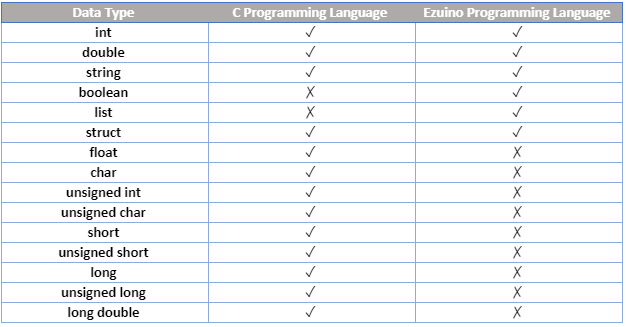
\includegraphics[scale=0.85]{figures/language_features/langf01.png}
\label{lf01}
\end{figure}
\subsubsection*{Bitwise Operators}
In the C programming language, six of its data types, signed and unsigned int char and long, supports for bit manipulation. %The following datatypes are char, int and long (signed and unsigned).
%The different bitwise operators can be found in figure \ref{lf02}:
%\begin{figure}[H]
%\centering
%\caption{Bitwise Operation comparison Arduino C and Ezuino}
%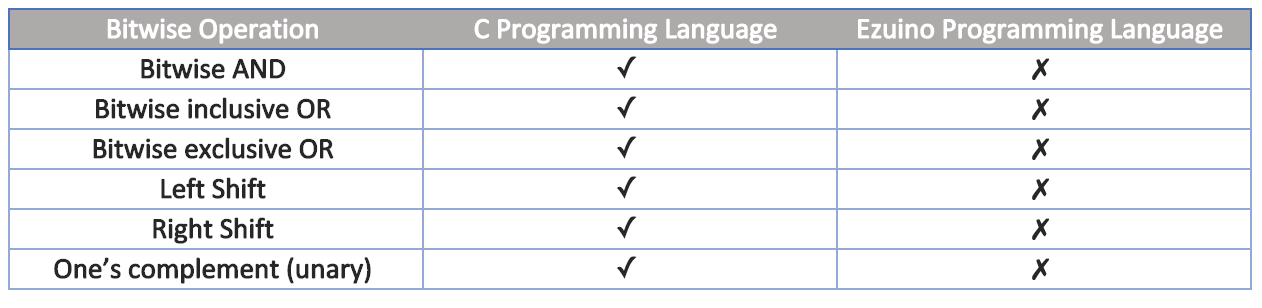
\includegraphics[scale=0.60]{figures/language_features/langf02.png}
%\label{lf02}
%\end{figure}
The reason why the Ezuino Programming language is not using the bitwise operations is that this may require a deeper understanding of how data structures work and require a more in-depth knowledge, which our target group shouldn’t be forced to learn. For our target group this increases readability by increasing the overall simplicity.
\subsubsection*{Logical Operators}
The logical operator is an expression, which is used to express logic in a programming language, and usually returns a boolean expression in the form of true or false. \\
As all three logical operators “AND” “OR” and “!” are an important part to define simple logical expressions, the Ezuino programming language has inherited all the functionality of the C programming language, although we have chosen to change the syntax. To increase writability through expressivity we have chosen to use “and” and “or” instead of \&\& and || that is used in C.\\
\begin{figure}[H]
\centering
\caption{Logical Operation comparison between Arduino C and Ezuino}
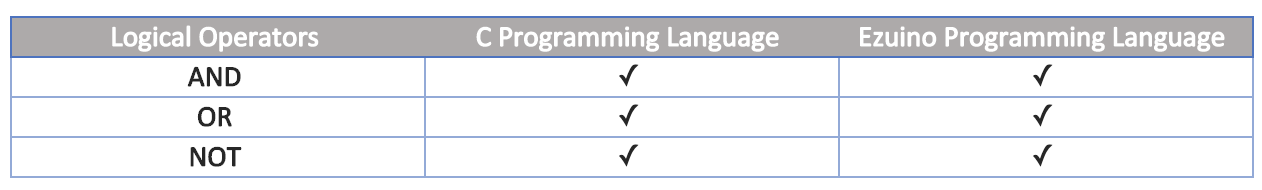
\includegraphics[scale=0.80]{figures/language_features/langf03.png}
\label{lf03}
\end{figure}
\subsubsection*{Relational Operators}
Relational operators define a relationship between two entities, and returns a boolean value.
The Ezuino programming language inherits all the features of C, as with the same case as the Logical Operators, relational operators are an important part of the programming language logic. We have chosen to keep the same relational operators as their syntax is very close with the mathematical notations. Compared to C, there will be differences in the equality operator, in ezuiono the syntax will be "=" instead of "==" in C. The different assignment syntax is chosen for its resemblance to mathematical notations in order to increase readability for people unfamiliar with code.
\begin{figure}[H]
\centering
\caption{Relational Operation comparison between Arduino C and Ezuino}
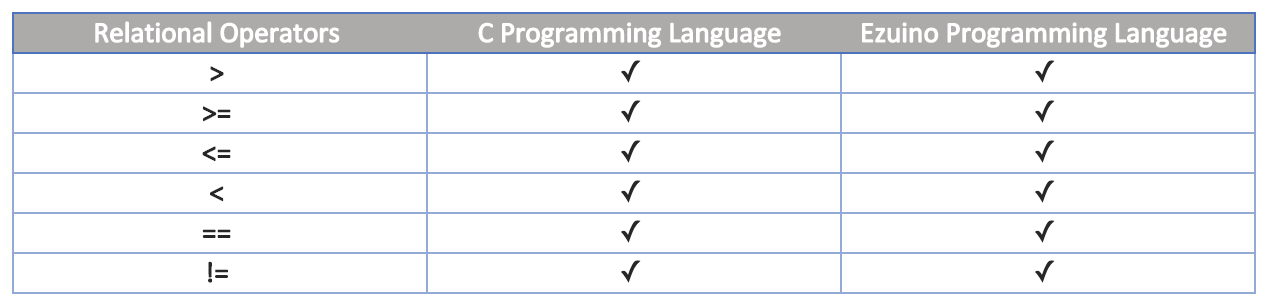
\includegraphics[scale=0.80]{figures/language_features/langf04.png}
\label{lf04}
\end{figure}

\subsubsection*{Arithmetical Operators and Negate}
Arithmetic operators are a necessity for every programming language.
Compared to C we have chosen to not include the modulo operator as it is a fairly programming specific operator not used commonly regular math. Furthermore, the orthogonality in Ezuino makes it possible to define other arithmetic operators as functions if necessary. The modulo operator is easily implemented as a function in our language. Considering these two points, we decided against implementing modulo as an operator.
The "-" sign will also work as negate, converting minus to plus and plus to minus. The functionality of this operator should be fine for people new to programming compared to modulus since it is often used in relatively basic mathematics.
\begin{figure}[H]
\centering
\caption{Arithmetical Operation comparison between Arduino C and Ezuino}
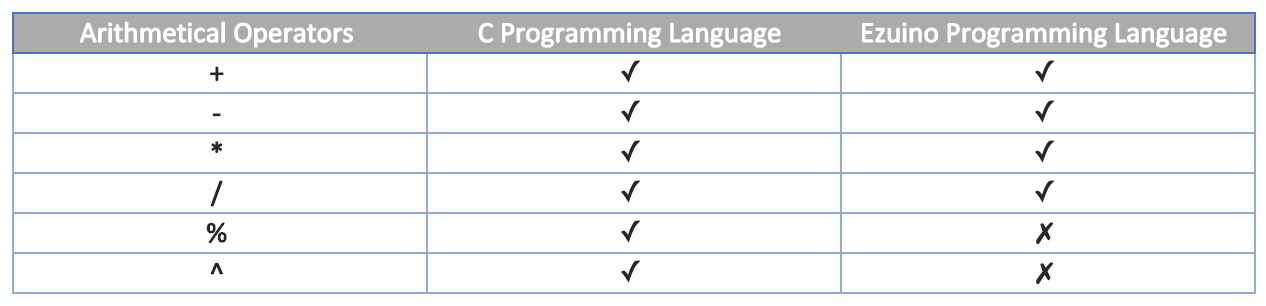
\includegraphics[scale=0.80]{figures/language_features/langf05.png}
\label{lf05}
\end{figure}

\subsubsection*{Pointer Operators}
As described in the problem analysis, most people have difficulty understanding the pointers and address systems, as it requires a sophisticated understanding of how the computer system works. Therefore, it has been decided not to include pointers in the Ezuino programming language. This also prevents most problems in aliasing increasing reliability.
\subsubsection*{Assignment Operators}
A way to assign a value to a variable is essential in any programming language Ezuino has also kept this feature. The syntax will be the one often seen as the mathematical notation for assignment “:=”. Other assignment operators in Arduiono C do several operations at once and while these are nice features we regard them as could have features, as they are not essential.
%\begin{figure}[H]
%\centering
%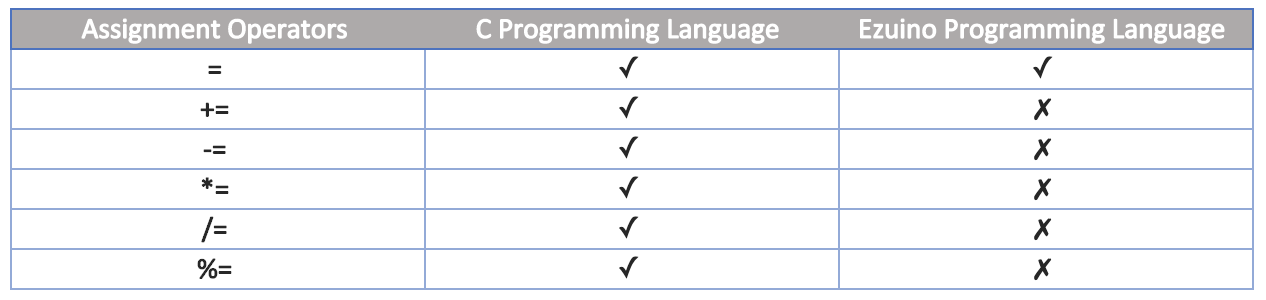
\includegraphics[scale=0.60]{figures/language_features/langf07.png}
%\caption{Assignment Operation comparison between C and Ezuino Programming Language}
%\label{lf07}
%\end{figure}
\subsubsection*{Control Flow}
In the C programming language, control flow statements of a programming language specify the order, in which computations get performed. To add an example, we can use a while loop. The while loop will keep running until a specific condition has not been met. For an example, if an Arduino is set to measure the outside temperature, and the Arduino executes a set of code, while the temperature is below its 20 degrees, the body of the loop will keep running until the temperature rises above 20 degrees. \\
\\
This is the general idea behind control flow. Control flow is a statement which executes of which result is being made as to which of two or more path to follow in a running program. \\
\\
To keep the most essential control flow structures we have chosen to keep the if else commands. We have not chosen to keep else if as it is more niche and if else can cover the same use cases if the use for it is absolutely necessary. This increases overall simplicity at the cost of reduced expressivity.
\\
In regards to loop structures the “while loop” will be the primary loop structure in Ezuono. Although the “for loop” and “do while loop” increase writability people can still do everything they need to in a “while loop”.
%\begin{figure}[H]
%\centering
%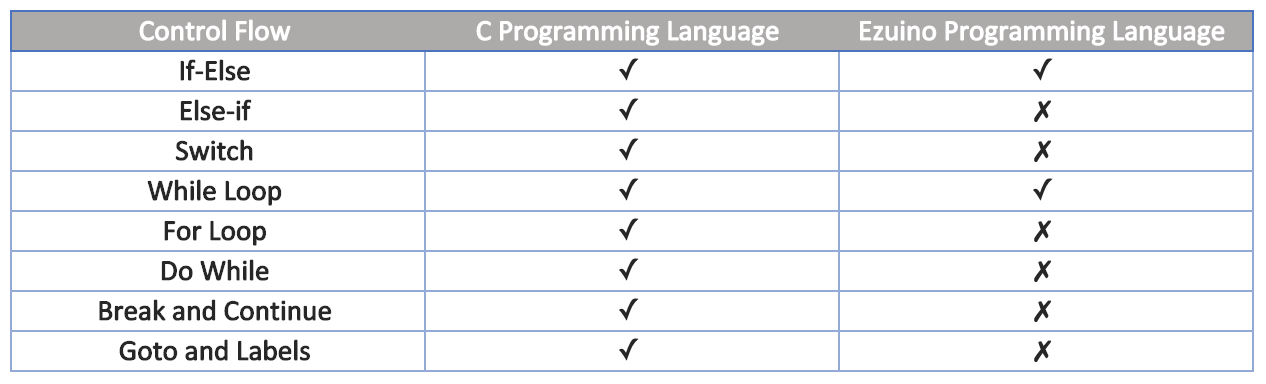
\includegraphics[scale=0.60]{figures/language_features/langf08.png}
%\caption{Control Flow comparison between C and Ezuino Programming %Language}
%\label{lf08}
%\end{figure}
\subsubsection*{Functions and Program Structure}
Functions in the C programming language is commonly used to task large code into smaller, reusable tasks. This enables the users to build and use the function which they have made, instead of writing all the code over again. A right style Arduino C program generally consist of a lot of minor functions, rather than having one significant function.
The basic Arduino functions should also be available in Ezuino, in order to communicate with the Arduino hardware. The ones we plan to implement as a proof of concept are Digital.Read, Digital.Write, Analog.Read, Analog.Write, Pin.Mode, delay, delayMicroseconds, Serial.print Serial.begin and Serial.end. The syntax in Ezuino will be the same albeit without “.” between keywords as we felt that this gave the impression of being object oriented.
\begin{figure}[H]
\centering
\caption{Functions and Program Structure comparison between Arduino C and Ezuino}
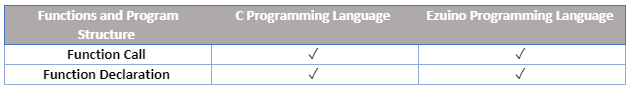
\includegraphics[scale=0.80]{figures/language_features/langf10.png}
\label{lf10}
\end{figure}
When defining the legal program structure there were three options we considered. \\ \\
\subsubsection{Option 1: Using global scope as main}
The global scope could be treated as the main function in Ezuino. This would mean everything inside the global scope should be regarded as legal statements. One of problems with this approach would be that statements and functions could be in arbitrary order. This could easily decrease readability if used improperly.
This would also require that the users would have to implement a while loop to have the same effect as Arduiono’s standard loop method, which is often necessary in Arduiono programs.
\begin{lstlisting}[caption={Program structure where global scope work as main}, label={lf10}]
int a := 5

func myfunc() {
	a := 8 + 2
}

a := 4
myfunc()
int b := 18
a := b*a

func otherfunc() {
	int c := 321
}

while(true) {
	otherfunc()
}
\end{lstlisting}

\subsubsection{Option 2: Having a main that works as a setup requiring the user to implement his own control structure}
If every statement should be inside main and function declaration should be outside, code would be relatively more orderly and easier to read.
This would however also require that the users implement a while loop if they needed repetition.
\begin{lstlisting}[caption={}, label={}]
func main() {
	int a := 5
	a := 4
	myfunc()
	int b := 10
	a := b*a
	
	while(true) {
		otherfunc()
	}
}

func myfunc() {
	int a := 8 * 2
}

func otherfunc() {
	int c := 321
}
\end{lstlisting}

\subsubsection{Option 3: Using arduino setup and loop but making loop optional}
Using the same setup method as Arduino is both relatively easy to read as the option 2, but also semantically reminds the user that a repetition is usually needed for arduino devices by giving it a place that is suitable for grouping such code.
\begin{lstlisting}[caption={Program structure similar to Arduino but where loop is optional}]
func Setup() {
	int a := 5
	a := 4
	myfunc()
	int b := 10
	a := b*a
}

func Loop() {
	otherfunc()
}

func myfunc() {
	int a := 8 * 2
}

func otherfunc() {
	int c := 321
}
\end{lstlisting}

\subsubsection{Chosen program structure for Ezuino}
Because option 2 and 3 both are relatively easier to read than option 1 and because option 3 semantically makes more sense, we chose option 2. Loop should also be optional to follow the design philosophy that extra syntax requirement that decrease writability and are unfriendly to people new to code should not be included.

\subsubsection*{Additional Constructs}
Single line comments will also be possible in Ezuino through \#, as comments are essential for reading code. Print will be available as print have multiple uses and are essential for simple debugging. End of statements will be without ; compared to C in order to increase writability, since it is easier not having to write the extra syntax. Requiring ; also encourages several compound statements on the same line, which reduces readability.
\begin{figure}[H]
\centering
\caption{Additional Constructs comparison Arduino C and Ezuino}
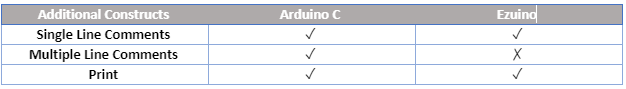
\includegraphics[scale=0.80]{figures/language_features/langf09.png}
\label{lf09}
\end{figure}

\subsection*{Casting}
With the Ezuino language it might be necessary to do casts from one type to another.
The print method should only accept the type string. To make sure that the user really wants to cast, casts have been made explicit.
That means if a user wants to use the print method on an integer, the integer firstly has to be cast to a string in order to print it.
Likewise, casts to the same type cannot be done. The reasoning for this is that it is important to know which types the variables has. If the user isn't aware of the types, it might be difficult to implement the functionality which user wants.\\
%The reason for not including casting from String to other data types is that this requires parsing of the string and as such is not a cast that makes sense.\\
The reason for not including casting from String to other data types is that this would require parsing and is not the same as casting. Since parsing strings to other data types have many practical uses but is slightly more time consuming and complex than parsing it should be included in Ezuino if there is enough time.  \\
When casting from boolean to integer false will equal 0 and true will equal 1.
In table \ref{tab:cast-overview}, the entire casts can be seen.
\begin{table}[H]
\centering
\begin{tabular}{lllll}
To\textbackslash From & String   & Integer      & Double       & Boolean      \\
String                & $\times$ & $\checkmark$ & $\checkmark$ & $\checkmark$ \\
Integer               & $\times$ & $\times$     & $\checkmark$ & $\checkmark$ \\
Double                & $\times$ & $\checkmark$ & $\times$     & $\checkmark$ \\
Boolean               & $\times$ & $\checkmark$ & $\times$     & $\times$    
\end{tabular}
\caption{List over casts in Ezuino. Casts marked with $\checkmark$ are valid, $\times$ marks invalid casts}
\label{tab:cast-overview}
\end{table}
\subsection*{Language design criteria and language feature overview}
After having described what the language design criteria is, the choice of every planned feature of Ezuino has been explained in comparison to C and what effect they should have on the language design criteria.
\begin{figure}[H]
\centering
\caption{An overview on language features of Ezuino overview and their effect on the language design criteria}
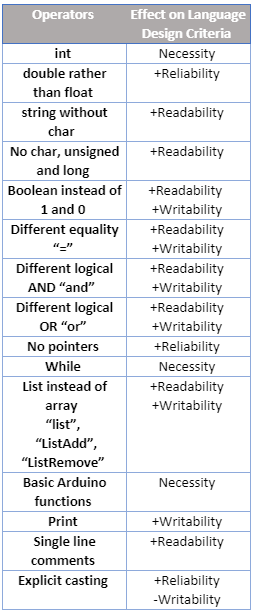
\includegraphics[scale=0.80]{figures/language_features/Operators-and-effect-on-language-criteria.png}

\label{feature-overview}
\end{figure}
\section{Contextual Restraints}
\subsection*{Static vs Dynamic Scope Rules}
Scope rules declare what bindings are used during execution of a procedure.
When an function is statically scoped it means that it saves the function and variable environment at declaration time. So even if the variables or functions it uses are changed, the function itself will not be changed since it uses the environment from when it was declared. Most programming languages today uses static scope rules (\cite{syntax-and-semantics}, p 85). 
\subsection*{Static vs Dynamic Type Binding }
The type of an declaration can be inferred at compile time (static type binding), or run times (dynamic type binding). Static type binding requires the programmer to declare the type when declaring a variable, while dynamic type binding binds a type to the variable when it is first assigned a value. Static type checking is the type binding most commonly used today(\cite{conceptsOfProgrammingLanguages}, p 228). \\ 
It has several advantages over dynamic type binding
\begin{itemize}
    \item It has more reliable at error detection. Since an variable has not been declared with a type in dynamic binding, there is no type check the first time the variable is assigned.
    \item The implementation is more complex and runs slower. Languages with dynamic type binding must use an run time descriptor to ensure that the variable assigned in run-time has enough storage.
    The execution is also slower since type checking has to be done while executing and cannot be done at compile time.
    \item Since the type of variables are only known at execution time Dynamic Type Binding is only suited for interpreters, since it is not possible to generate machine instruction without knowing the data types.
\end{itemize}


\subsection*{Block Structure }
When an variable is declared the declaration type and identifier is saved in an identification table, also known as an symbol table. \\
The organization of the symbol table depends on the languages block structure, which is the textual relationships of blocks in programs. \\
Block structures are divided between three types, monolithic, flat and nested (\cite{compilers-and-intepreters}, chapter 5).
In a monolithic block structure the entire program is one block. This means that there may be no variables with the same identifier.
In a flat block structure, there is distinction between
\begin{itemize}
    \item Local scope. Applied occurrence of locally declared identifiers are restricted to a particular block.
    \item Other declaration are global in scope. Applied occurrences of locally declared identifiers are allowed anywhere in the program. 
    In effect, the program as a whole is a block, enclosing all the other blocks.
\end{itemize}
Finally nested blocks are a block structure where blocks may be nested in other blocks. 
\begin{itemize}
    \item Declarations in the outermost block are global in scope. We say that the outermost block 
is at scope level 1.

\item Declarations inside an inner block are local to that block. Every inner block is completely enclosed by another block. If enclosed by the outermost block, we say that the inner block is at scope level; if enclosed by a level-2 block, we say that the inner block is scope level 3; and so on.
\end{itemize}

\subsection*{Contextual Restraints For Ezuino}
The target group for Ezuino is people with no prior coding experience [\ref{targetedGroup}]. We have chosen Static Dynamic Scope rules since it is more commonly used today and to be consistent with static type binding which we have also chosen for Ezuino. The biggest advantage if we had chosen dynamic type binding is its increased ease of cost in terms of training new programmers that are not familiar with basic data types. While this fit our target group the disadvantage of less reliable error detection could lead to about the same amount of frustration if not worse, for someone inexperienced in writing code. Furthermore it harder to implement a dynamic type checker. \\
In terms of block structure even though Monolithic block structure is the simplest concept to understand for new programmers, it is less flexible especially regarding the readability of control statements. Declaring variables in the block they are used, makes for more readable code. For the same reason nested block structure are more suitable than flat block structure because it allows multiple nested control statements to have their variables declared inside their block. 

The Ezuino language has partially nested block structures, as variables can be declared in every block. This means that every block has its own scope, including `if`, `while`, `else` and `function` blocks
Functions are limited to be declared in the global scope. This ensures that functions cannot be defined within other functions. The structure of a function is somewhat complex as a function can be very long and if Ezuino had nested block structures for functions it can be hard to distinguish which functions are available at a given time.

The reason for not limiting variables is that the structure of variable declarations is simple. The only issue in doing this is that variables are limited to that scope. While this might confuse users, at the same time this also give the users the flexibility for users declaring the variables.
The variable declarations have been limited to be at the very top of a block. In that way the variables are always found at the same place. It takes inspiration from Pascal in that way that pascal must define variables in a special block. While the special block was good for separation, it seemed excessive to explicitly make a special block structure for declarations. As such the Ezuino language still requires the user to specify variables in the beginning, but without the special block.
\section{The Scanner, Parser and Chosen Parser Generator Tool}
This chapter will explain what the job of the scanner and parser is in compiler construction, what a parsing generator tool is, the theories it implements and which parser generator we chose for Ezuino.
% \begin{figure}[H]
%\centering
%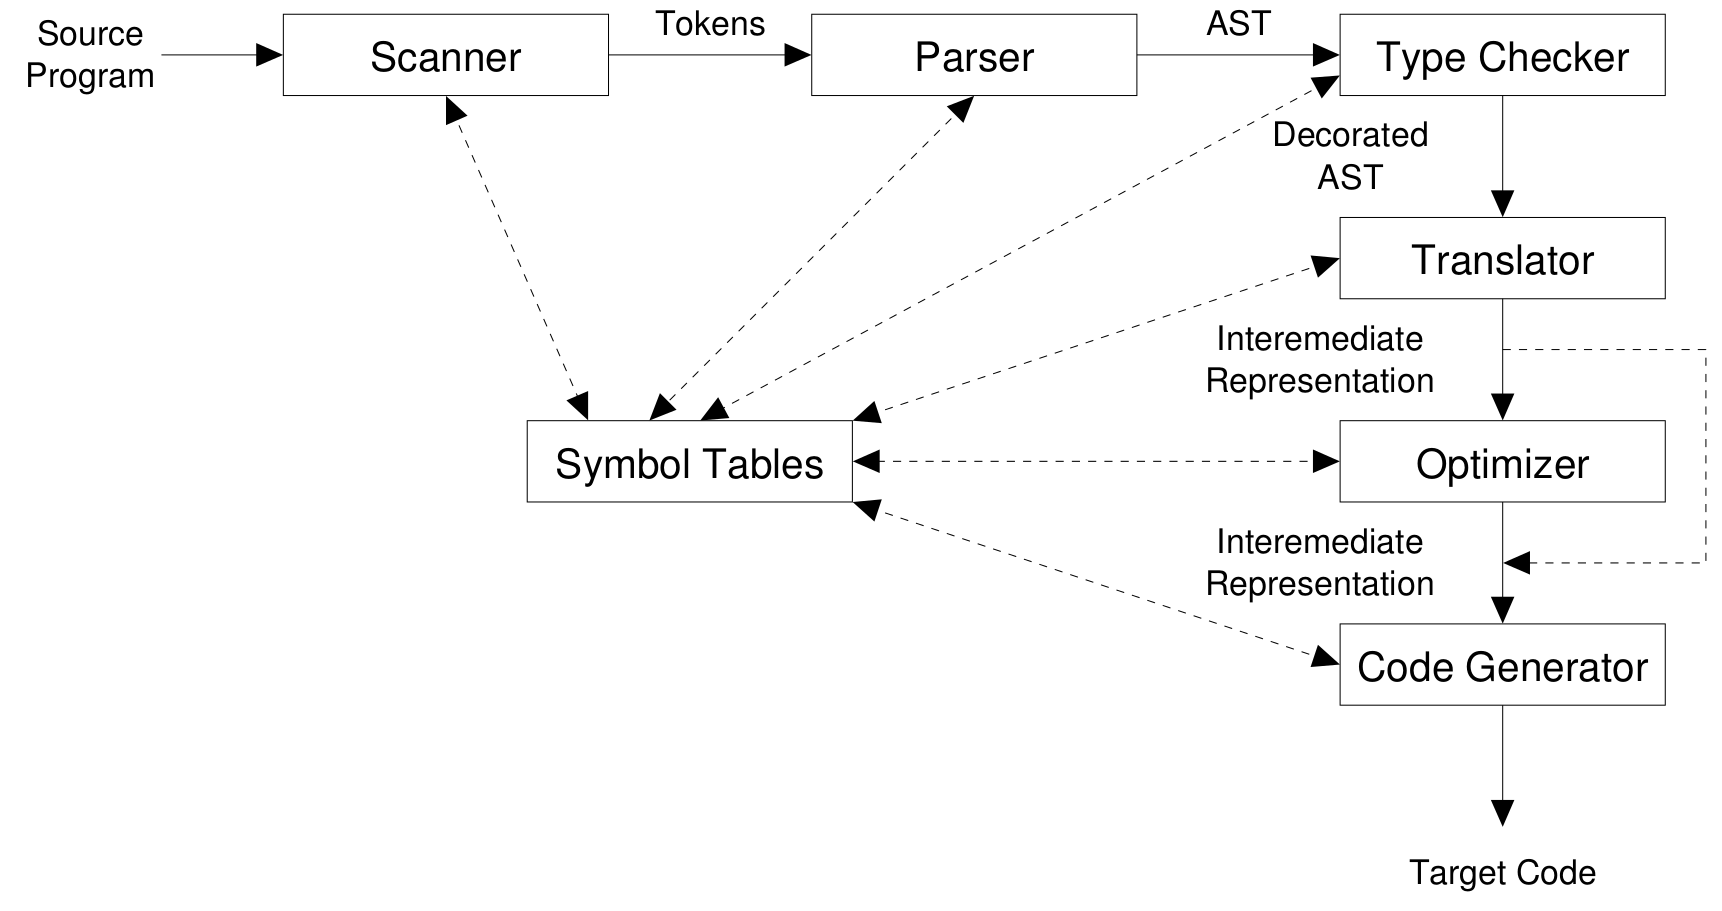
\includegraphics[width=\textwidth]{figures/compiler-process.png}
%\caption{Organization of a compiler, Source: Fischer \cite{crafting-a-compiler} }
%\label{syntax-overview}
%\end{figure}
%This chapter will contain the decisions we made in regards to the compiler of our language, as well as our arguments for making these decisions.

\subsection{The Scanner}
A scanner, also called a Lexer, is the first processing step of a programming language. It reads the input text, ignores comments, and turns it into a compact and uniform format known as tokens.
A scanner is most often created through declarative programming, often done with the parser generator tool. That it is declarative means to create the scanner you tell the generator what tokens to recognize in regular expressions and let the generator do the implementation.

\label{parsing-subsubsection}
\subsection{Parsing}
Just like the scanner, a parser is often created through declarative programming by a parsing generator tool. The purpose of the parser is to read tokens generated by the scanner and generate phrases according to a context-free grammar file, which then checks are syntactically correct. If there is an error it either reports it, attempts to repair it (to create a syntactically valid program), or tries to recover from the error in order to continue parsing. Besides verifying the syntax of a program is valid, the parsing should also generate a concrete syntax tree. This concrete syntax tree can then create an abstract syntax tree used by other parts of the compiler.

\subsection{Choosing a parser generator tool}
In order to understand what the parser generator tool does, it is necessary to explain the theory behind parsing techniques. When constructing a parser one of two strategies is usually used to recognize and construct tokens based on the context-free grammar of the language, namely top-down parsing and bottom-up parsing. It is also necessary to keep in mind what kind of parsing the generated parser does. Finally, the different generator tools create a concrete parse tree and how easy they are to convert to an abstract syntax tree should also be taken into consideration.
\subsubsection*{Top-down and bottom-up parsing}
Given a starting symbol and a set of rules, a top-down parser will start reading its input as a long line of tokens from a scanner. In general, the tokens are read from left to right\footnote{Unless your source language is a language that writes from right to left, of course}, and are afterwards derived from the starting symbol using a leftmost-derivation of the non-terminals through the grammatical rules\cite{conceptsOfProgrammingLanguages}.\\
\\
An example of a top-down parsing is the recursive descent parser, which is built from a collection of subprograms that each produces its own top-down parse tree generator. The subprograms in itself are recursive and the recursive descent parser will only create one subprogram for every non-terminal it can find in the user-generated grammar\cite{conceptsOfProgrammingLanguages}.\\
\\
A bottom-up parser is the other method of parsing. A bottom-up parser also reads a line of tokens, but rather than starting at the top and deriving to terminals, it builds non-terminals based on the symbols it reads, by performing a rightmost-derivation in accord with the grammatical rules, until it reaches the starting symbol\cite{conceptsOfProgrammingLanguages}.\\
\\
\subsubsection{Parsing trees and abstract parsing tree}
The end goal of either strategy is to generate a parse tree\footnote{Sometimes known as a concrete syntax tree (a CST)}, which represents the syntactic structure of the program source code. The parse tree is defined by an input string and a grammar, or in this case for the project, a context-free-grammar \\

\begin{figure}[H]
\centering
\caption{Parse tree example}
\label{exampleparse}
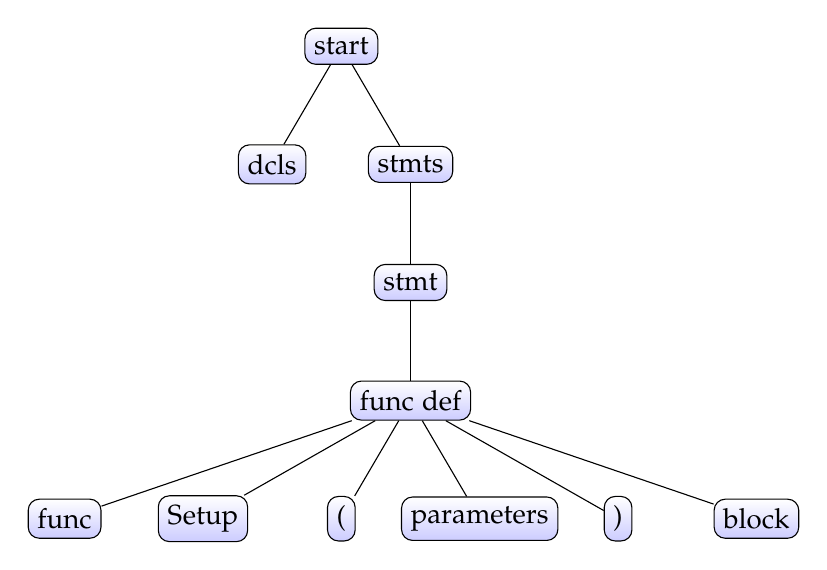
\begin{tikzpicture}[sibling distance=5em,
  every node/.style = {shape=rectangle, rounded corners,
    draw, align=center,
    top color=white, bottom color=blue!20}]]
  \node {start}
    child { node {dcls} }
    child { node {stmts}
      child { node {stmt}
        child { node {func def}
          child { node {func} }
          child { node {Setup} }
          child { node {(} }
          child { node {parameters} }
          child { node {)} } 
          child { node {block} } } } };
\end{tikzpicture}
\end{figure}

The picture in figure \ref{exampleparse} shows a parse tree, where the highest node, which is “start” has 2 child nodes which are “dcls” and “stmts”. It will then traverse further down until it reaches an end. \\
An abstract syntax tree provides the advantage that removes non-essential elements of the syntax. E.g. the colons, equality signs etc. and provides a structure which can be altered and annotated to make sure that contextual analysis is performed correctly.
The abstract syntax tree is more an idea since it is very dependent on the construction of the programming language. The structure is a representation of the essential information from the parse tree, with inessentials removed (braces, parentheses, etc.). In an abstract syntax tree the entire source program should be stored in the structure and using this structure alone, the compiler programmer should be able to reconstruct the entire source program. If one cannot recreate the source program, essential structures have been removed.\cite{crafting-a-compiler}
A common method of creating an abstract syntax three is through the visitor pattern. The visitor pattern is an object oriented pattern provided by the GoF Design Patterns book.
It solves the problem of defining a new operation without changing the classes of the elements on which it operates.
The visitor therefore makes it easy to handle methods in a class in a specific context. A visitor simply has to specify how to visit all the nodes in the tree.
\subsubsection{Types of parsing}
\subsubsection*{LL-parsing}
The LL parser (Left to right and left most derivation) is a parser that parses its input from left to right while using a top-down parsing technique. It is usually denoted as LL(k), where k is a greater than or equal to 0, where the k signifies the amount of lookahead tokens the parser can look at\cite{conceptsOfProgrammingLanguages}.

\subsubsection*{LR-parsing}
The LR parser (Left to right and rightmost derivation) is a parser that parses its input from left to right, but unlike the LL(k) parser, the LR parser uses a bottom-up parsing technique and produces a rightmost derivation. Just as the LL(k) the k in the LR(k)-definition signifies the amount of tokens the LR will look ahead for\cite{conceptsOfProgrammingLanguages}. LR-parsers usually have a magnitude of either 0 or 1 (LR(0) or LR(1)), as LR(1)-parsers already use many resources to parse a given input, and even higher magnitudes severely slow down the entire program.

\subsubsection*{LALR- and LALR(1) parsing}
The LALR(k) parser is a parser that utilizes the same parsing strategy as the LR(k) parser (bottom-up), but with a different way to generate a parse table, the part of an LR parser that instructs the parser how to react to a given input. Usually, an LALR-parser is of magnitude 1, as an LALR(1)-parser is more powerful than an LR(0)-parser, but not as resource intensive as an LR(1)-parser. It should be noted, that the LR(1)-parser is still more powerful than the LALR(1)-parser, which is why it is still in use\cite{crafting-a-compiler}.

\subsubsection*{Table driven LL(K) parsing}
The table driven LL(k) parser uses a similarity analysis to the generated grammar so that when it starts with pushing the start symbol into the stack, the parser would try to find a match of symbols from the input and when found, put the symbol into the top of the stack\cite{crafting-a-compiler}. This is nice for when you have a big code block and you want the parsing to be automated by using a stack.

\subsubsection{Considered parser generators and choice}
In this subsection we will list the different parser generator tools we tried and which one we chose. \\

\begin{table}[h]
\centering
\begin{tabular}{@{}ll@{}}
\toprule
\textbf{Parser} & \textbf{Type} \\ \midrule
ANTLR           & LL(*)         \\
Bison           & LALR(1)       \\
GOLD            & LALR(1)       \\
SableCC         & LALR(1)       \\ \bottomrule
\end{tabular}
\label{parser_table}
\end{table}

\noindent
Out, of all the possible generators we researched, we seriously considered two of them. \\
\\
One of them was using a tool called Flex, an open-source implementation of the Lex program for generating a scanner and Bison, a Yacc-based parser generator, for generating a parser. To get familiar with the tools, we attempted to implement an infix calculator. It was not particularly complex to use the tools together, but it was not always clear why an error occurred, due to the unfamiliar naming scheme that bison and flex use. \\
Flex and Bison only target C and C++, meaning we would also have to write the rest of our compiler in C or C++. While both C and C++ are powerful languages, it is also hard to write well, and it takes a long time to write code that works. \\
The other alternative which is also the one we chose, was ANTLR4. ANTLR4 targets Java is comparative more efficient and which we were more familiar with. The naming convention used by the ANTLR4 parser made more sense as well, and the context free grammar format for ANTLR4 was also slightly more practical. Another advantage of ANTLR4 was that it also generates a base abstract syntax tree interface that can be extended by the programmer. This helped setting up the structure of the abstract syntax tree. ANTLR4 is also more popular and was therefore also easier to find documentation for.








%\subsection{Type Checker}
%During the Type Checker, the types of variables and functions are checked. By saving what the type of each variable is, it is possible to check whether the variables are correctly used. This might be to check if an assignment of the variable is possible or not. This phase is not limited to only type checking. The phase is meant for all the semantic analysis, which is dependant on the compiler programmers. This might include checking for double declaration, declaration before usage, etc.
%The result of running the Type Checker is a decorated Abstract Syntax Tree. The abstract syntax tree might is decorated with types but might have other information associated with it, depending on the compiler.

%\subsection{Translator and optimizer}
%The translator phase of the compiler takes the decorated abstract syntax tree and makes it into an intermediate representation. The reason for this is that it might be easier to deal with the intermediate representation in the code generation phase.
%The translator phase is optional as code can be generated directly from the abstract syntax tree.
%The output result is simply the intermediate representation.
%The optimizer phase is optional. This is where the code is optimized and bottlenecks are removed. It is done with the idea in mind that you can reduce the size of the code and also reduce the running time of the program. 

%\begin{itemize}
%    \item Peekhole optimization
%    \item Constant folding
%    \item Common sub-expression elimination
%    \item Code motion
%    \item Dead code elimination
%\end{itemize}{}

%In order to make more efficient code one might eliminate dead variables like this:
%\begin{verbatim}
%func int magicNumber() {
%    int t
%    t := 40 * 20 - 100 / 4
%    return 42
%}
%\end{verbatim}
%where t is a dead variable.




%\subsection{Code Generator}
%In the Code Generator phase, the target code is generated. Depending if the compiler generated the intermediate representation or not, the source here is either the intermediate representation or the abstract syntax tree directly. The implementation here is very dependant on the target language as some target languages uses registers directly or stack based machines.

%ANTLR4 only provides a context syntax tree (also known as a parse tree) of the source program. The parse tree from ANTLR is the direct translation of the source program parsed by ANTLR using the grammar. The nodes in the parse tree is thus directly related to the tokens provided in the grammar.

%To convert the parse tree to an abstract syntax tree, you have to convert every single node to the alternative.
%Doing this with ANTLR requires a great overview of both datastructures and the visitor which can be generated by ANTLR. The visitor is an ANTLR specific implementation of the visitor pattern.



%\subsection{Symboltable}
%While the visitor pattern provides a way of handling the nodes in the abstract syntax tree there might be necessary to keep some information when transitioning trough the nodes. This can simply be kept in a private attribute for simple information. However there might be some difficulty dealing when scope rules. Thus it might be nessecary with a symboltable.
%A symboltable is datastructure that XX TODO. Whenever opening a new scope the symboltable needs to know and thus declares a new scope. Whenever exiting a scope, close the scope. 
%You end up with a decorated abstract syntax tree.

%\subsubsection{Codegeneration}
%earing the end, of the compiler, after doing all the contextual analysis, you end up with a decorated syntax tree which has made sure that everything lives up to the programming language that has been defined. Now it’s time for code generation.
%Here there can be multiple code generators as it simply can follow the visitor pattern in order to generate the code. This is the point where the designer of the compiler decides what the resulting language of the compiler should be. It could be C, Assembly, etc. It depends on what the programming language is designed for. Sometimes it might be necessary to make some predefined code in order to support the structures and functionality of the programming language.
%A good approach might be to create an intermediate language if you want to compile multiple high-level programming languages to a low-level programming language. In that way instead of making many compilers from D => B, E => B, D => C, E => C, you can simply create one compiler from the high-level language to the intermediate language. Similarly, if you want to output to multiple low level languages, you simply need to add another compiler from the intermediate language to the new low-level language. In that way, instead of making high-level \* low-level number of compilers, you simply have to make Highlevel \+ Low-level number of compilers. It adds abstraction but might also add complexity if either the source language or the destination language has structures which are hard or impossible to implement. Some examples of compilers with intermediate languages are Java and C\#. Java compiles to Java Bytecode which is the instruction set of the Java Virtual Machine. C\# compiles to Common Intermediate Language which is then run on the Common Language Runtime.

%\subsection{Compiler}
%A compiler is a translator from a source language to a target language.
%Depending on the compiler, the compiler may generate one or more of these: Pure Machine Code, Augmented Machine Code or Virtual Machine Code.[Ref Fischer]
%In this report the source language is the language "Ezuino" and the target language is Jasmin [TODO].

%\subsubsection{Jasmin}
%Jasmin is an assembler for the Java Virtual Machine. It provides takes ASCII syntax of the Java Bytecode and makes into the binary Java Bytecode. [Fischer cap 10.2.2]. 


\section{Syntax Specification}
\subsection{Reserved words \& Keywords}
In the Ezuino programming language, a reserved keyword is vital to prevent users to overwrite, define and use keywords, which is used in the programming language already. In case that a user tries to define a variable or function named a reserved keyword, they will receive an error, which will be thrown into the error handler. The error handler will then tell the users, where and which reserved keyword they used where. The reserved keywords are words primarily used in the Java and C programming language. The following reserved keywords can be found in table \ref{reservedKeywordsList}.

\begin{table}[H]
\centering
\caption{Table of Reserved Keywords}
\begin{tabular}{llll}
if           & switch      & int         & boolean     \\
return       & AND         & OR          & true        \\
false        & int         & double      & main        \\
string       & while       & else        & Print       \\
DigitalWrite & DigitalRead & AnalogWrite & AnalogRead  \\
Delay        & DelayMicro  & PinMode     & SerialBegin \\
SerialEnd    & Setup       & Loop        & goto        \\
float        & for         & ArrayList   & List        \\
Collection   &             &             &            
\end{tabular}
\label{reservedKeywordsList}
\end{table}
\section{Introduction to Grammar}
This section will explain on how the grammar for the syntax language will be generated and the reason for why each part of the language was made as it is. 

\subsection{Context Free Grammar (ANTLR4)}
Context free grammar describes the syntax of the language. ANTLR4 which is the parser generator for this language has it's own version of EBNF (Extended Backus–Naur form) it uses to implement the syntax.
The different annotation used in order to express EBNF can be seen in the table below.
\begin{center}
\begin{tabular}{ |c|c| } 
 \hline
 ? & Zero or one occurrence\\ 
 \hline
 | & One or the other \\ 
 \hline
 * & Zero or more occurrence \\ 
 \hline
  + & One or more occurrence \\ 
 \hline
\end{tabular}
\end{center}


\lstinputlisting[caption={EBNF for Ezuino}, label={code:ebnf},numbersep=5pt,language={[Plain]TeX}]{sections/language_design/syntax/Ezuino.g4}
\subsection{Program Example}
This section will provide some example code, which was created in the early iteration of the project development, in the Ezuino programming language syntax. The first code snippet is in figure \ref{ex01}, which is one the largest general code examples written for the Ezuino language. This code snippet has been a part of the unit tests in several areas of the compiler. \\
From lines 1-10, we declare the variables in all the types, the Ezuino language support. \\
Line 13-22, we assign the previously assigned variables some values equal to their respective type. \\
Starting from line 23, the findMedium function will take the input of the four integer declarations made earlier. Inside the function, we test the variable declarations in functions and assignment, using ret on line 28.\\
At the end of the function, we take the sum of the input variables on line 29 by dividing them with 4. \\
In the last part of the example code starting from line 32 we define another function, named asd. Inside asd function, we have a while loop and a if else statement. We also call the findMedium function as the right hand part of an assignment. Both the while loop and if else statements uses boolean variable declarations or statments.
\begin{lstlisting}[caption={Example full program}, label={ex01}]
int testOne
int testTwo
int testThree
int testFourOne
int testFourTwo
int testFour
int medium
double doubleTest
boolean boolTest1
boolean boolTest2

func Setup() {
	testOne := 1
	testTwo := 20
	testThree := 30
	testFourOne := 10
	testFourTwo := 10
	testFour := testFourOne + testFourTwo
	doubleTest := 23.23
	boolTest1 := true
	boolTest2 := false
	stringTest := "Hello world!"
}

func int findMedium(int testOne, int testTwo, int testThree, int testFour) {
	int ret
	ret := 1
	return (testOne + testTwo + testThree + testFour)/4
}

func int asd() {
	while (testOne < 10 OR testOne < 10) {
		testOne := testOne+1
	}
	if (testOne >= testTwo AND testOne != testFour) {
		testTwo := testTwo + testTwo
	}
	else {
		testTwo := testTwo * testTwo + testTwo
	}
	medium := findMedium(testOne, testTwo, testThree, testFour)
	return medium
}
\end{lstlisting}
\noindent\newline
Following is a short example of a recursive program in Ezuino.
\begin{lstlisting}[caption={A small recursive program}, label={ex02}]
int y
func int add(int x, int t) {
	if (t == 0) {
	    return 0
	}
	y := add(x, t-1) + 1
	return y
}
func main() {
	int r
	int a
	int b
	a := 5
	b := 8
	r := add(a, b)
}
\end{lstlisting}
\noindent\newline

\chapter{Semantics}
\label{semantics}
\section{Abstract Syntax for Ezuino}
At this stage, we got the syntax made, and we have a general idea of the language. The next step is to construct semantics for the Ezuino programming language. This chapter will go through each semantic rule, in categorized. 
Before we can start on semantics, we need a table, to provide an overview of the short names in each semantic. This can be  reviewed in figure \ref{semCat}.
\begin{figure}[H]
\centering
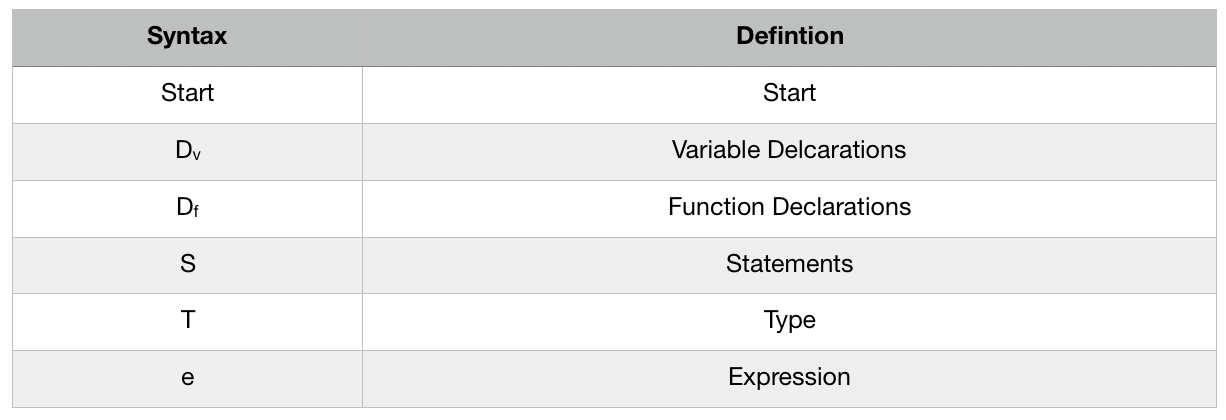
\includegraphics[scale=0.75]{figures/semantics/categories.png}
\caption{Table of Reserved Keywords}
\label{semCat}
\end{figure}

\section{Structural Operation Semantics}
The operational semantics are the rules that give our syntax meaning, and without them it would be impossible to make a working language, as a given syntax wouldn't have a clearly defined functionality. For this reason, we will define the operational semantics in this section.

There are 2 different ways of describing semantics of a language. Big-step semantics and small-step semantics. While they are equivalent, there are some advantages and disadvantages to both of them. The big-step semantics evaluates the whole expression from the start to the end expression. Small-step semantics may only evaluate part of the expression one step at a time. The disadvantage of small-step semantics is that it can be daunting to both write and read.

We have decided to make our operational semantics a small-step semantic, as a small-step semantic ruleset is easier to extend in the case of a new feature compared to a big-step semantic ruleset. This means that it would be possible to add parallelity, if we realize that we need it at a later date.

\subsection{Environment-Store Model}
One of the ways we can describe how the Ezuino compiler must handle and store variables, we must just the Environment Store Model (ESM). There are differnet mechanism inside the ESM, and some we will go through the essentials before starting on the semantics. First, we have the location, which marks the location of every variable value in the program. The location keeps track of a variable in the environment $env_v$.
To continue with the ESM, we got the partial function named Store (Sto), which for an instance of the program binds its storage location to values, which are contained within. An example of this, is that if we want to find the value of a specific variable, in this case named x, we write $"sto \  env_v \ x"$.
Next we have the run-time s tack named envl. The runtime stack is a list of pairs ($env_v$, $env_p$).
On figure \ref{evnstoreexmp}, the ESM can be reviewed.
\begin{figure}[H]
\centering
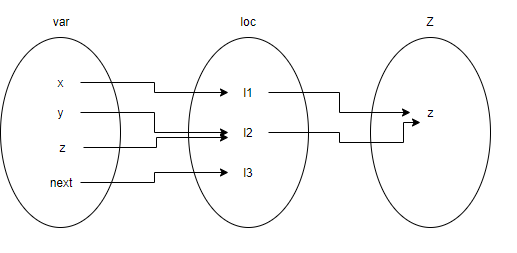
\includegraphics[scale=0.75]{figures/evnstore.png}
\caption{Environment Store Example}
\label{evnstoreexmp}
\end{figure}

\subsection{Arithmetic Expressions}
In the following table, it should be noted that most transitions will be on the form \( \langle envl, sto, a \rangle \Rightarrow_e \langle envl', sto', v \rangle \). This is supposed to be read as "By evaluating a in accord with the runtime stack and the store like an expression, a is evaluated to the value v, and the runtime stack and store is updated

\begin{longtable}[c] { r c }
  \centering
  
  [VAR] & \( envl, sto \vdash x \Rightarrow_e v \) \\
  & if \(env_v x = l \) \\
  & and \(sto \ l = v \) \\
  & where \(envl = (env_v, env_p) : envl' \) \\
  &  \\

  [DCL] & \( 
    \dfrac{ \langle D_V, envl[x \mapsto l][next \mapsto \text{new} \ l], sto \rangle \Rightarrow_{DV} \langle envl', sto \rangle}
    { \langle T x, envl, sto \rangle \Rightarrow_{DV} \langle envl', sto \rangle } \) \\
  & \\

  [PARENT-1] & 
    \( \dfrac { \langle e, envl, sto \rangle \Rightarrow_e \langle e', envl', sto' \rangle }
      { \langle (e), envl, sto \rangle  \Rightarrow_e \langle (e'), envl', sto' \rangle } \) \\
  & \\

  [PARENT-2] & 
    \( \langle (v), envl, sto \rangle \Rightarrow_e \langle v, envl, sto \rangle \) \\
  & \\

  [PLUS-1] & 
    \( \dfrac { \langle e_1, envl, sto \rangle \Rightarrow_e \langle e_1', envl', sto' \rangle )}
      {\langle e_1 + e_2, envl, sto \rangle \Rightarrow_e \langle e_1' + e_2, envl', sto' \rangle } \) \\
  & \\

  [PLUS-2] & 
    \( \dfrac { \langle e_2, envl, sto \rangle \Rightarrow_e \langle e_2', envl', sto' \rangle }
      {\langle v_1 + e_2, envl, sto \rangle  \Rightarrow_e \langle e_1 + e_2', envl', sto' \rangle } \) \\
  & \\

  [PLUS-3] & 
    \( \langle v_1 + v_2, envl, sto \rangle \Rightarrow \langle v, envl, sto \rangle \) \\
  & where \( v = v_1 + v_2\) \\
  & \\

  [MINUS-1] & 
    \( \dfrac { \langle e_1, envl, sto \rangle \Rightarrow_e \langle e_1', envl', sto' \rangle }
      {\langle e_1 - e_2, envl, sto \rangle \Rightarrow_e \langle e_1' - e_2, envl', sto' \rangle } \) \\
  & \\

  [MINUS-2] & 
    \( \dfrac { \langle e_2, envl, sto \rangle \Rightarrow_e \langle e_2', envl', sto' \rangle }
      {\langle v_1 - e_2, envl, sto \rangle \Rightarrow_e \langle v_1 - e_2', envl', sto' \rangle } \) \\
  & \\

  [MINUS-3] & 
    \( \langle v_1 - v_2, envl, sto \rangle \Rightarrow \langle v, envl, sto \rangle \) \\
  & where \( v = v_1 - v_2\) \\
  & \\

  [MULT-1] & 
    \( \dfrac { \langle e_1, envl, sto \rangle \Rightarrow_e \langle e_1', envl', sto' \rangle }
      {\langle e_1 * e_2, envl, sto \rangle \Rightarrow_e \langle e_1' * e_2, envl', sto' \rangle } \) \\
  & \\

  [MULT-2] & 
    \( \dfrac { \langle e_2, envl, sto \rangle \Rightarrow_e \langle e_2', envl', sto' \rangle }
      {\langle v_1 * e_2, envl, sto \rangle \Rightarrow_e \langle v_1 * e_2', envl', sto' \rangle } \) \\
  & \\

  [MULT-3] & 
    \( \langle v_1 * v_2, envl, sto \rangle \Rightarrow \langle v, envl, sto \rangle \) \\
  & where \( v = v_1 * v_2\) \\
  & \\

  [DIV-1] & 
    \( \dfrac { \langle e_1, envl, sto \rangle \Rightarrow_e \langle e_1', envl', sto' \rangle }
      {\langle e_1 / e_2, envl, sto \rangle \Rightarrow_e \langle e_1' / e_2, envl', sto' \rangle } \) \\
  & \\

  [DIV-2] & 
    \( \dfrac { \langle e_2, envl, sto \rangle \Rightarrow_e \langle e_2', envl', sto' \rangle }
      {\langle v_1 / e_2, envl, sto \rangle \Rightarrow_e \langle v_1 / e_2', envl', sto' \rangle } \) \\
  & \\

  [DIV-3] & 
    \( \langle v_1 / v_2, envl, sto \rangle \Rightarrow \langle v, envl, sto \rangle \) \\
  & where \( v = \dfrac{ v_1 }{ v_2 } \) \\
  & \\

  [NEGATION-1] & 
    \( \dfrac { \langle e_1, envl, sto \rangle \Rightarrow_e \langle e_1', envl', sto' \rangle }
      {\langle -e_1, envl, sto \rangle \Rightarrow_e \langle -e_1', envl', sto' \rangle } \) \\
  & \\

  [NEGATION-2] & 
    \( \langle -v_1, envl, sto \rangle \Rightarrow \langle v, envl, sto \rangle \) \\
  & where \( v = -v_1 \)\\
  & \\

  [NUM] & 
    \( n \Rightarrow v \) \\
  & \( \text{if } \mathcal{N} [[n]] = v \) \\

  \caption{Small-step semantics for arithmetic expressions}
\end{longtable}

\subsection{Boolean Expressions}
\begin{longtable}[c] { r c }
  \centering
  [NOT-1] & \( 
    \dfrac { \langle e, envl, sto \rangle \Rightarrow_e \langle e', envl', sto' \rangle }
      { \langle !e, envl, sto \rangle \Rightarrow_e \langle !e', envl', sto' \rangle } \)
  \\
  & \\

  [NOT-TRUE] & \( 
    \langle !v, envl, sto \rangle \Rightarrow_e \langle tt, envl, sto \rangle \)
  \\
  & if \( v = ff\) \\
  & \\

  [NOT-FALSE] & \( 
    \langle !v, envl, sto \rangle \Rightarrow_e \langle ff, envl, sto \rangle \)
  \\
  & if \( v = tt \) \\
  & \\

  [AND-1] & \( 
    \dfrac { \langle e_1, envl, sto \rangle \Rightarrow_e \langle e_1', envl', sto' \rangle }
      { \langle e_1 \ AND \ e_2, envl, sto \rangle \Rightarrow_e \langle e_1' \ AND \ e_2, envl', sto' \rangle } \)
  \\
  & \\

  [AND-2] & \( 
    \dfrac { \langle e_2, envl, sto \rangle \Rightarrow_e \langle e_2', envl', sto' \rangle }
      { \langle v_1 \ AND \ e_2, envl, sto \rangle \Rightarrow_e \langle v_1 \ AND \ e_2', envl', sto' \rangle } \)
  \\
  & \\

  [AND-3] & \( 
    \langle v_1 \ AND \ v_2, envl, sto \rangle \Rightarrow_e \langle tt, envl, sto \rangle \)
  \\
  & if \( v_1 \land v_2 \) \\
  & \\

  [AND-4] & \( 
    \langle v_1 \ AND \ v_2, envl, sto \rangle \Rightarrow_e \langle ff, envl, sto \rangle \)
  \\
  & if \( \neg(v_1 \land v_2) \) \\
  & \\

  [OR-1] & \( 
    \dfrac { \langle e_1, envl, sto \rangle \Rightarrow_e \langle e_1', envl', sto' \rangle }
      { \langle e_1 \ OR \ e_2, envl, sto \rangle \Rightarrow_e \langle e_1' \ OR \ e_2, envl', sto' \rangle } \)
  \\
  & \\

  [OR-2] & \( 
    \dfrac { \langle e_2, envl, sto \rangle \Rightarrow_e \langle e_2', envl', sto' \rangle }
      { \langle v_1 \ OR \ e_2, envl, sto \rangle \Rightarrow_e \langle v_1 \ OR \ e_2', envl', sto' \rangle } \)
  \\
  & \\

  [OR-3] & \( 
    \langle v_1 \ OR \ v_2, envl, sto \rangle \Rightarrow_e \langle tt, envl, sto \rangle \)
  \\
  & if \( v_1 \lor v_2 \) \\
  & \\

  [OR-4] & \( 
    \langle v_1 \ OR \ v_2, envl, sto \rangle \Rightarrow_e \langle ff, envl, sto \rangle \)
  \\
  & if \( \neg(v_1 \lor  v_2) \) \\
  & \\

  [EQUAL-1] & \( 
    \dfrac { \langle e_1, envl, sto \rangle \Rightarrow_e \langle e_1', envl', sto' \rangle }
      { \langle e_1 = e_2, envl, sto \rangle \Rightarrow_e \langle e_1' = e_2, envl', sto' \rangle } \)
  \\
  & \\

  [EQUAL-2] & \( 
    \dfrac { \langle e_2, envl, sto \rangle \Rightarrow_e \langle e_2', envl', sto' \rangle }
      { \langle v_1 = e_2, envl, sto \rangle \Rightarrow_e \langle v_1 = e_2', envl', sto' \rangle } \)
  \\
  & \\

  [EQUAL-3] & \( 
    \langle v_1 = v_2, envl, sto \rangle \Rightarrow_e \langle tt, envl, sto \rangle \)
  \\
  & if \( v_1 = v_2 \) \\
  & \\

  [EQUAL-4] & \( 
    \langle v_1 = v_2, envl, sto \rangle \Rightarrow_e \langle ff, envl, sto \rangle \)
  \\
  & if \( \neg(v_1 = v_2) \) \\
  & \\

  [NOT-EQUAL-1] & \( 
    \dfrac { \langle e_1, envl, sto \rangle \Rightarrow_e \langle e_1', envl', sto' \rangle }
      { \langle e_1 != e_2, envl, sto \rangle \Rightarrow_e \langle e_1' != e_2, envl', sto' \rangle } \)
  \\
  & \\

  [NOT-EQUAL-2] & \( 
    \dfrac { \langle e_2, envl, sto \rangle \Rightarrow_e \langle e_2', envl', sto' \rangle }
      { \langle v_1 != e_2, envl, sto \rangle \Rightarrow_e \langle v_1 != e_2', envl', sto' \rangle } \)
  \\
  & \\

  [NOT-EQUAL-3] & \( 
    \langle v_1 != v_2, envl, sto \rangle \Rightarrow_e \langle tt, envl, sto \rangle \)
  \\
  & if \( \neg(v_1 = v_2) \) \\
  & \\

  [NOT-EQUAL-4] & \( 
    \langle v_1 != v_2, envl, sto \rangle \Rightarrow_e \langle ff, envl, sto \rangle \)
  \\
  & if \( v_1 = v_2 \) \\
  & \\

  [GREATER-THAN-1] & \( 
    \dfrac { \langle e_1, envl, sto \rangle \Rightarrow_e \langle e_1', envl', sto' \rangle }
      { \langle e_1 > e_2, envl, sto \rangle \Rightarrow_e \langle e_1' > e_2, envl', sto' \rangle } \)
  \\
  & \\

  [GREATER-THAN-2] & \( 
    \dfrac { \langle e_2, envl, sto \rangle \Rightarrow_e \langle e_2', envl', sto' \rangle }
      { \langle v_1 > e_2, envl, sto \rangle \Rightarrow_e \langle v_1 > e_2', envl', sto' \rangle } \)
  \\
  & \\

  [GREATER-THAN-3] & \( 
    \langle v_1 > v_2, envl, sto \rangle \Rightarrow_e \langle tt, envl, sto \rangle \)
  \\
  & if \( v_1 > v_2 \) \\
  & \\

  [GREATER-THAN-4] & \( 
    \langle v_1 > v_2, envl, sto \rangle \Rightarrow_e \langle ff, envl, sto \rangle \)
  \\
  & if \( \neg(v_1 > v_2) \) \\
  & \\

  [GREATER-THAN-OR-EQUAL-1] & \( 
    \dfrac { \langle e_1, envl, sto \rangle \Rightarrow_e \langle e_1', envl', sto' \rangle }
      { \langle e_1 > = e_2, envl, sto \rangle \Rightarrow_e \langle e_1' > = e_2, envl', sto' \rangle } \)
  \\
  & \\

  [GREATER-THAN-OR-EQUAL-2] & \( 
    \dfrac { \langle e_2, envl, sto \rangle \Rightarrow_e \langle e_2', envl', sto' \rangle }
      { \langle v_1 > = e_2, envl, sto \rangle \Rightarrow_e \langle v_1 > = e_2', envl', sto' \rangle } \)
  \\
  & \\

  [GREATER-THAN-OR-EQUAL-3] & \( 
    \langle v_1 > = v_2, envl, sto \rangle \Rightarrow_e \langle tt, envl, sto \rangle \)
  \\
  & if \( v_1 \geq v_2 \) \\
  & \\

  [GREATER-THAN-OR-EQUAL-4] & \( 
    \langle v_1 > = v_2, envl, sto \rangle \Rightarrow_e \langle ff, envl, sto \rangle \)
  \\
  & if \( \neg(v_1 \geq v_2) \) \\
  & \\

  [LESS-THAN-1] & \( 
    \dfrac { \langle e_1, envl, sto \rangle \Rightarrow_e \langle e_1', envl', sto' \rangle }
      { \langle e_1 < e_2, envl, sto \rangle \Rightarrow_e \langle e_1' < e_2, envl', sto' \rangle } \)
  \\
  & \\

  [LESS-THAN-2] & \( 
    \dfrac { \langle e_2, envl, sto \rangle \Rightarrow_e \langle e_2', envl', sto' \rangle }
      { \langle v_1 < e_2, envl, sto \rangle \Rightarrow_e \langle v_1 < e_2', envl', sto' \rangle } \)
  \\
  & \\

  [LESS-THAN-3] & \( 
    \langle v_1 < v_2, envl, sto \rangle \Rightarrow_e \langle tt, envl, sto \rangle \)
  \\
  & if \( v_1 < v_2 \) \\
  & \\

  [LESS-THAN-4] & \( 
    \langle v_1 < v_2, envl, sto \rangle \Rightarrow_e \langle ff, envl, sto \rangle \)
  \\
  & if \( \neg(v_1 < v_2) \) \\
  & \\

  [LESS-THAN-OR-EQUAL-1] & \( 
    \dfrac { \langle e_1, envl, sto \rangle \Rightarrow_e \langle e_1', envl', sto' \rangle }
      { \langle e_1 < = e_2, envl, sto \rangle \Rightarrow_e \langle e_1' < = e_2, envl', sto' \rangle } \)
  \\
  & \\

  [LESS-THAN-OR-EQUAL-2] & \( 
    \dfrac { \langle e_2, envl, sto \rangle \Rightarrow_e \langle e_2', envl', sto' \rangle }
      { \langle v_1 < = e_2, envl, sto \rangle \Rightarrow_e \langle v_1 < = e_2', envl', sto' \rangle } \)
  \\
  & \\

  [LESS-THAN-OR-EQUAL-3] & \( 
    \langle v_1 < = v_2, envl, sto \rangle \Rightarrow_e \langle tt, envl, sto \rangle \)
  \\
  & if \( v_1 \leq v_2 \) \\
  & \\

  [LESS-THAN-OR-EQUAL-4] & \( 
    \langle v_1 < = v_2, envl, sto \rangle \Rightarrow_e \langle ff, envl, sto \rangle \)
  \\
  & if \( \neg(v_1 \leq v_2) \) \\
  & \\
  \caption{Small-step semantics boolean expressions}
\end{longtable}
\subsection{Boolean Expressions}
\begin{table}[H]
    \centering
    \begin{longtable}[c] { r c }
    \begin{tabular}{@{}c@{}} 
    [ASS1] &
    \\
    \\
    \end{tabular}
  \begin{tabular}{@{}c@{}}   \( <x := a, sto, env_l> \Rightarrow (sto[l -> v], envl) \)  \\ \( env_v,sto \vdash n \Rightarrow v \)
  \\ \( env_v,sto \vdash n \Rightarrow v \)
  \end{tabular}
        
 \end{longtable}
    \caption{Small-step semantics for boolean assignment expressions}\label{tab:my_label}
\end{table}
        
\begin{table}[H]
    \centering
    \begin{longtable}[c] { r c }
        
        [IF-ELSE-TRUE] & \( \dfrac{\langle \texttt{if} \ b \ \texttt{then} \ S_1 \ \texttt{else} \ S_2,\ s \rangle \Rightarrow \langle S_1,\ s\rangle}{if\ s\vdash b \rightarrow_b tt} \) \\[4ex]
        
        [IF-ELSE-FALSE] & \( \dfrac{\langle \texttt{if} \ b \ \texttt{then} \ S_1 \ \texttt{else} \ S_2,\ s \rangle \Rightarrow \langle S_2,\ s \rangle}{if\ s\vdash b \rightarrow_b ff} \) \\[4ex]
        
        [IF-TRUE] & \( \dfrac{\langle \texttt{if} \ b \ \texttt{then} \ S_1,\ s \rangle \Rightarrow \langle S_1,\ s \rangle}{if \ s\vdash b \rightarrow_b tt} \) \\\\
        
        [IF-FALSE] & \( \dfrac{\langle \texttt{if} \ b \ \texttt \ S_1,\ s \rangle \Rightarrow s}{if\ s\vdash b \rightarrow_b ff} \) \\[4ex]
        
 \end{longtable}
    \caption{Small-step semantics for boolean if statement}\label{tab:my_label}
\end{table}
        
\begin{table}[H]
    \centering
    \begin{longtable}[c] { r c }
        
        [WHILE] & \( \langle \texttt{while(} \ b\texttt{) \{} S \texttt{\}},\ s \rangle \Rightarrow \langle \texttt{if} \ b \ \texttt{then} (S\texttt{;while (} b \texttt{) \{} S\texttt{\}}) \texttt{else skip,}\ s\rangle) \) \\[4ex]
        
 \end{longtable}
    \caption{Small-step semantics for boolean while statements}\label{tab:my_label}
\end{table}
        
\begin{table}[H]
    \centering
    \begin{longtable}[c] { r c }
    
        [END] & END\\
    \end{longtable}
    \caption{Small-step semantics for end}\label{tab:my_label}
\end{table}
%% SCOPE RULES INERT HERE
\section{Type System Semantics}
The Ezuino programming language data types is only primitive types. This is denoted in future references as :
\begin{table}[H]
    \centering
    \begin{longtable}[c] { r c }
      
        \( { T_{TP} = (string,\ bool,\ double,\ integer)} \) \\
    \end{longtable}
    \caption{}\label{s-empty}
\end{table}





\subsection{Type Environment}
%\begin{table}[H]
%    \begin{center}
%    \begin{longtable}[c] { r c }
%        [Example_{test}] 
%        & 
%        \( \dfrac{T E(T x; D_v, T E) = T E(D_v, T E[x 7 \mapsto T])} 
%        {T E(T x; D_v, T E) = T E(D_v, T E[x 7 \mapsto T])} \) 
%        \\ \\
%        & 
%        \( {where \ T \ \epsilon \ T_{primitive} \ \textbackslash \ %\{void,\ bool,\ text,\ number\}} \)
%    \end{longtable}
%    \caption{}\label{s-empty}
%        \end{center}
%\end{table}
Updating a type environment with empty have no effect on the type environment.
\begin{table}[H]
    \centering
    \begin{longtable}[c] { r c }
        $[Update_{empty}]$ & 
        \( {TE(\epsilon, TE) = TE} \) \\
    \end{longtable}
    \caption{}\label{s-empty}
\end{table}


Declaring a variable updates the type environment with the variables type.
\begin{table}[H]
    \begin{center}
    \begin{longtable}[c] { r c }
        $[Update_{D_v}]4$ 
        & 
        \( {T E(T \ x;\ D_v, T E) = T E(D_v,\ T E[x \mapsto T])} \) 
        \\ \\
        & 
        \( {where \ T \ \epsilon \ T_{pt}} \)
    \end{longtable}
    \caption{}\label{s-empty}
        \end{center}
\end{table}

Declaring a function updates the type environment with the functions formal parameters and return type.
\begin{table}[H]
    \begin{center}
    \begin{longtable}[c] { r c }
        $[Update_{D_f}]$ 
        & 
        \( T E(T \ f(T_1 x_1,\ ...,\ T_k x_k)S \ D_f
,\ T E) = T E(D_f
,\ T E[f  \mapsto  (T_1,\ ...\, T_n \ × \ T_r)])
( \) 
    \end{longtable}
    \caption{}\label{s-empty}
        \end{center}
\end{table}

\subsubsection*{Expressions}
Expressions are the core of most programming operations. Ezuino supports parenthesis, arithmetic and logical expressions. Since casting is explicit integers and doubles are not compatible and their type rules are therefore separated despite both using type rules operating on numbers. As it was argued in \ref{language-features} string also supports the equality and concatenation operation as these are seen as essential features of strings.
\begin{table}[H]
    \begin{center}
    \begin{longtable}[c] { r c }
        $[Parenthesis] $
        & 
        \( \dfrac{T E  \vdash  e  :  T}{T E  \vdash  (e)  :  T} \) 
        \\ \\
        & 
        \( {where \ T \ \epsilon \ \{ bool,\ string,\ int,\ double\}} \)
    \end{longtable}
    \caption{}\label{s-empty}
        \end{center}
\end{table}
 
\begin{table}[H]
    \begin{center}
    \begin{longtable}[c] { r c }
        $[ArithInt_{e}]$ 
        & 
        \( \dfrac{TE \vdash e_{1} :  int \ \ TE \vdash e_{2} : int} 
        {\ TE \vdash e_{1} \ op \ e_{2} : int} \) 
        \\ \\
        & 
        \( {where \ op \ \epsilon \ \{+, \ -, \ /, \ *\} } \)
    \end{longtable}
    \caption{}\label{s-empty}
        \end{center}
\end{table}
\begin{table}[H]
    \begin{center}
    \begin{longtable}[c] { r c }
        $[ArithDouble_{e}]$ 
        & 
        \( \dfrac{TE \vdash e_{1} : double \ \ TE \vdash e_{2} :  double} 
        {\ TE \vdash e_{1} \ op \ e_{2} : double} \) 
        \\ \\
        & 
        \( {where \ op \ \epsilon \ \{+, \ -, \ /, \ *\} } \)
    \end{longtable}
    \caption{}\label{s-empty}
        \end{center}
\end{table}
\begin{table}[H]
    \begin{center}
    \begin{longtable}[c] { r c }
        $[IntRelation_{e}]$ 
        & 
        \( \dfrac{T E  \vdash  e_1  :  int \ T E  \vdash  e_2  :  int}{T E  \vdash  e_1 \ op \ e_2  :  bool} \) 
        \\ \\
        & 
        \( {where \ op \ \epsilon \ \{<,\ >,\ <=,\ >=,\ =,\ !=\}} \)
    \end{longtable}
    \caption{}\label{s-empty}
        \end{center}
\end{table}

\begin{table}[H]
    \begin{center}
    \begin{longtable}[c] { r c }
        $[DoubleRelation_{e}]$ 
        & 
        \( \dfrac{T E  \vdash  e_1  : double \ T E  \vdash  e_2  :  double}{T E  \vdash  e_1 \ op \ e_2  :  bool} \) 
        \\ \\
        & 
        \( {where \ op \ \epsilon \ \{<,\ >,\ <=,\ >=,\ =,\ !=\}} \)
    \end{longtable}
    \caption{}\label{s-empty}
        \end{center}
\end{table}
\begin{table}[H]
    \begin{center}
    \begin{longtable}[c] { r c }
        $[StringRelation_{e}]$ 
        & 
        \( \dfrac{T E  \vdash  e_1  :  string \ TE  \vdash  e_2  :  string }{TE  \vdash  e_1 \ op \ e_2  :  bool} \) 
        \\ \\
        & 
        \( {where \ op \ \epsilon \ \{=, \ !=\}} \)
    \end{longtable}
    \caption{}\label{s-empty}
        \end{center}
\end{table}


\begin{table}[H]
    \begin{center}
    \begin{longtable}[c] { r c }
        $[Logical_{e}]$ 
        & 
        \( \dfrac{T E  \vdash  e_1  :  string \ TE  \vdash  e_2  :  string }{T E  \vdash  e_1 \ op \ e_2  :  bool} \) 
        \\ \\
        & 
        \( {where \ op \ \epsilon \ \{=,\ !=\, AND,\ OR,\ !,\ <,\ <=,\ >,\ >= \}} \)
    \end{longtable}
    \caption{}\label{s-empty}
        \end{center}
\end{table}

\begin{table}[H]
    \begin{center}
    \begin{longtable}[c] { r c }
        $[Concat]$ 
        & 
        \( \dfrac{TE \vdash  e_1  :  string \ \ TE  \vdash  e_2  :  string }{TE \vdash  e_1 \ op \ e_2  :  string} \) 
                 \\ \\
        & 
        \( {where \ op \ \epsilon \ \{+ \}} \)
    \end{longtable}
    \caption{}\label{s-empty}
        \end{center}
\end{table}

\begin{table}[H]
    \begin{center}
    \begin{longtable}[c] { r c }
        $[NegInt_{e}]$ 
        & 
        \( \dfrac{T E  \vdash  e_1  :  int}{T E  \vdash  -e_1  :  int} \) 
    \end{longtable}
    \caption{}\label{s-empty}
        \end{center}
\end{table}

\begin{table}[H]
    \begin{center}
    \begin{longtable}[c] { r c }
        $[NegDouble_{e}]$ 
        & 
        \( \dfrac{T E  \vdash  e_1  :  double}{T E  \vdash  -e_1  :  double} \) 
    \end{longtable}
    \caption{}\label{s-empty}
        \end{center}
\end{table}

\begin{table}[H]
    \begin{center}
    \begin{longtable}[c] { r c }
        $[Not_{e}]$ 
        & 
        \( \dfrac{T E  \vdash  e_1  :  bool}{T E  \vdash  !e_1  :  bool} \) 
    \end{longtable}
    \caption{}\label{s-empty}
        \end{center}
\end{table}

\begin{table}[H]
    \begin{center}
    \begin{longtable}[c] { r c }
        $[Var]$ 
        & 
        \( {T E  \vdash x  :  T} {where \ T E(x)=\ T} \)
         \\ \\
        & 
        \( {and \ T \ \epsilon \ \{bool,\ string,\ int,\ double\}} \)
    \end{longtable}
    \caption{}\label{s-empty}
        \end{center}
\end{table}
In a function declaration the return type is specified and the types for the formal parameters are saved in the type environment. Afterwards there can be statements and other function declarations. \\
Every statement in the function declaration must be OK in regards to the declared return type. This means that return statements in if and else statements as well as return statements in the function declaration body must return the declared return type. \\ 
Functions declared in a function declaration must be well typed as well.
\begin{table}[H]
    \begin{center}
    \begin{longtable}[c] { r c }
        $[FuncDcl]$ 
        & 
        \( \dfrac{TE' \vdash S : OK \ \ TE \vdash D_{f}: OK} 
        {T E \vdash T_r \ f(T_1 \ x_1,\ ...,\ T_n,\ x_n)S D_f : OK} \) 
        \\ \\
        & 
        \( {where \ TE' = TE[r \mapsto T_r]} \)
    \end{longtable}
    \caption{}\label{s-empty}
        \end{center}
\end{table}

In a while loop the expression must be a bool type while the statement inside the the while loop must be OK.
\begin{table}[H]
    \begin{center}
    \begin{longtable}[c] { r c }
        $[While]$ 
        & 
        \( \dfrac{T E  \vdash e  :  bool \ T E \vdash S : OK}{T E \vdash while(e) \ S : OK} \)

    \end{longtable}
    \caption{}\label{s-empty}
        \end{center}
\end{table}

Check if and else expression are OK, and if they are OK then also make sure the statements of the if and else statements are OK.
\begin{table}[H]
    \begin{center}
    \begin{longtable}[c] { r c }
        $[If - else]$ 
        & 
        \( \dfrac{T E  \vdash e  :  bool \ T E \vdash S_1 : OK \ OK \ T E \vdash S_2 : OK}
        {T E \vdash if(e) \ S_1 \ else \ S_2 : OK} \)

    \end{longtable}
    \caption{}\label{s-empty}
        \end{center}
\end{table}

The return statement is only correct when its expression type is the same as the function type. The function return type is found in the type environment
\begin{table}[H]
    \begin{center}
    \begin{longtable}[c] { r c }
        $[Return]$ 
        & 
        \( \dfrac{T E  \vdash e  :  T}{T E \vdash return \ e : OK} \)
         \\ \\
        & 
        \( {if \ TE(r) = T } \)

    \end{longtable}
    \caption{}\label{s-empty}
        \end{center}
\end{table}








\subsection{Blocks}
Blocks can be referred to as the body of if-else statenents, while statements and functions. Each block has a specific scoping, which is handled by the Symbol Table as described in \ref{Block_Structure_Symbol_Tables}. The first symbol table will start with a global scope and add a scope for each new block that is being created. In table \ref{block}, we can see that we can look back to the previously known variable declarations.
\begin{table}[H]
    \begin{center}
    \begin{longtable}[c] { r c }
        $[Block]$ 
        & 
        \( \dfrac{TE' \vdash S : OK} 
        {TE \vdash D_v S : OK} \) 
        \\ \\
        & 
        \( {where \ TE' = TE(D_v, TE)} \)
    \end{longtable}
    \caption{}\label{block}
        \end{center}
\end{table}

Table \ref{active-block} is the active block which is the block we’re currently in. Unlike table \ref{block}, it cannot know its previous blocks, however, it is the one which are current for each block.
\begin{table}[H]
    \begin{center}
    \begin{longtable}[c] { r c }
        $[Block_{current}]$ 
        & 
        \( \dfrac{TE \vdash D_{v} : OK \ TE \vdash S : OK} 
        {TE \vdash current \ D_{v} \ S \ end  :  OK} \)
    \end{longtable}
    \caption{}\label{active-block}
        \end{center}
\end{table}

\section{Structural Operation Semantics}
\subsection{Environment-Store Model}
One of the ways we can describe how the Ezuino compiler must handle and store variables, we must just the Environment Store Model (ESM). There are differnet mechanism inside the ESM, and some we will go through the essentials before starting on the semantics. First, we have the location, which marks the location of every variable value in the program. The location keeps track of a variable in the environment {env_v}.
To continue with the ESM, we got the partial function named Store (Sto), which for an instance of the program binds its storage location to values, which are contained within. An example of this, is that if we want to find the value of a specific variable, in this case named x, we write "sto env_v x".
\chapter{Implementation}
This chapter will go through implementing the Ezuino programming language. The programming language is done, and we can group the different implementation topics. First, we will go through the build Abstract Syntax Tree (AST) visitor class and then move to type checker, where we provide each node in the AST a type. Then we will go through the different visitors and code generation visitors. Finally, we will go through the error handler, which provides an error overview for the users.
\section{Type checker}
The type checker implements the semantic rules of Ezuino specified in chapter \ref{semantics}. \\
We split the type checker into two visitors TypeCheckerVisitor and ReturnStatementVisitor. TypeCheckerVisitor checks that the condition in a boolean statement has the correct type and that expressions are legal. ReturnStatementVisitor ensures that the actual returned value of a program matches the type defined in the function declaration.
The way TypeCheckerVisitor type checks expressions is through a setup where every expression node extends that inherits from an interface called ITypeNode. The ITypeNode interface requires that every child class have the method for getting and setting a type attribute. When type checking happens, we then compare each node through the checkType method.
\begin{lstlisting}[caption={checkType function}, label={code:TC:checkType}]
private void checkType(ITypeNode leftNode, ITypeNode rightNode) {
    Type leftType = leftNode.getType();
    Type rightType = rightNode.getType();
    if (leftType == null) {
        System.err.println("Left type null!");
        return;
    }
    if (rightType == null) {
        System.err.println("Right type null!");
        return;
    }
    if (leftType != rightType) {
        errorHandler.typeMismatch(leftNode, rightNode);
    }
}
\end{lstlisting}
\noindent\newline

The boolean condition is checked in an if- and else statements.
\begin{lstlisting}[caption={Visit if statement node}, label={code:TC:if}]
$$@Override
public void visit(If_stmtNode node) {
    node.getExpr().accept(this);
    node.getIfBlock().accept(this);
    if (node.getElseBlock() != null) {
        node.getElseBlock().accept(this);
    }
    checkSpecificType(node.getExpr(), Type.BOOL);
}
\end{lstlisting}
\noindent\newline

An example of type checking expressions. When an additive expression is reached both nodes are type checked.
\begin{lstlisting}[caption={Visit additive expression node}, label={code:TC:Additive}]
$$@Override
public void visit(AdditiveExprNode node) {
    node.getLeftNode().accept(this);
    node.getRightNode().accept(this);
    checkType(node.getLeftNode(), node.getRightNode());
    node.setType(node.getLeftNode().getType());
    if (node.getType().equals(Type.BOOL) ||
        node.getType().equals(Type.STRING) && node.getOperator().equals("-")) {
        errorHandler. invalidOperatorForType(node.getOperator(), node.getType());
    }
}
\end{lstlisting}
\noindent\newline

In a unary expression it is also necessary to check that the operations performed are done with legal types. This is done through an switch case so it is easy to extend if more unary expressions needs to be added in the future. 
\begin{lstlisting}[caption={Visit unary expression node}, label={code:TC:Unary}]
$$@Override
public void visit(UnaryExprNode node) {
    node.getNode().accept(this);
    Type nodeType = node.getNode().getType();
    node.setType(nodeType);
    String nodeOperator = node.getOperator();
    boolean printErr = false;
    if ("-".equals(nodeOperator)) {
        printErr = nodeType.equals(Type.BOOL) || nodeType.equals(Type.STRING);
    } 
    else if ("!".equals(nodeOperator)) {
        printErr = !nodeType.equals(Type.BOOL);
    }
    if (printErr) {
        errorHandler.invalidOperatorForType(nodeOperator, nodeType);
    }
}
\end{lstlisting}
\noindent\newline

When a return statement is returned it is set to its expression, this is important for type checking the return statement with the function declaration later in ReturnStatementVisitor.
It is also here that return in void functions is implemented. If a return statement has no value,we assume it to be a void function. This in practice makes the return key-word a way to preemptively end void functions.
\begin{lstlisting}[caption={Visit return statement node}, label={code:TC:return}]
$$@Override
public void visit(Return_stmtNode node) {
    Type nodeType = Type.VOID;
    AExpr expression = node.getReturnExpr();
    if (expression != null) {
        expression.accept(this);
        nodeType = expression.getType();
    }
    node.setType(nodeType);
}
\end{lstlisting}
\noindent\newline

This is the ReturnStatementVisitor. When a function is declared the type, it was declared as is temporarily saved in a symbol table. When a return statement is reached, the return statements type is compared with a type of the last function that was declared which was saved in the symbol table within that scope. This ensures that if there are several nested function declarations, the return type is compared to the most recent “active” scope.
\begin{lstlisting}[caption={Visit function definition node in return statement visitor}, label={code:ReturnCheck:FuncDef}]
$$@Override
public void visit(Func_defNode node) {
    symtable.openScope();
    symtable.enterSymbol(FUNC_DEF_ID, node);
    node.getBlockNode().accept(this);
    symtable.closeScope();
}
\end{lstlisting}
\noindent\newline

\begin{lstlisting}[caption={Visit return statement node in return statement visitor}, label={code:ReturnCheck:returnstmt}]
$$@Override
public void visit(Return_stmtNode node) {
    Func_defNode funcdefnode = (Func_defNode) symtable.retrieveSymbol(FUNC_DEF_ID);
    checkType(funcdefnode, node);
}
\end{lstlisting}
\noindent\newline

\section{Checking that return are guaranteed}
If an function is not a void function, it should only be legal if it is guaranteed that it will reach an return statement. This means that if there is no return statement in the scope of the definition body, it must be because there is an if- and else block in the scope of the body where every if statement and the else statement have an return statement. 

\begin{figure}[H]
\centering
\frame{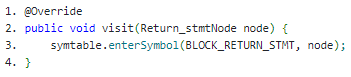
\includegraphics[scale=1.0]{figures/implementation/typeCecker/3-3-return-stmt-enter-symbol-table.png}}
\caption{If a return statement is encountered it, it is noted for the current scope.}
\label{lf05}
\end{figure}

\begin{figure}[H]
\centering
\frame{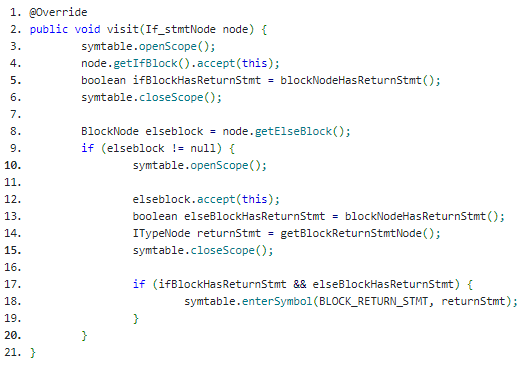
\includegraphics[scale=1.0]{figures/implementation/typeCecker/3-2-ifstmt-return-check.png}}
\caption{If an return statement in an if else block is guaranteed, it is noted for the current scope.} 
\label{lf05}
\end{figure}

 \begin{figure}[H]
\centering
\frame{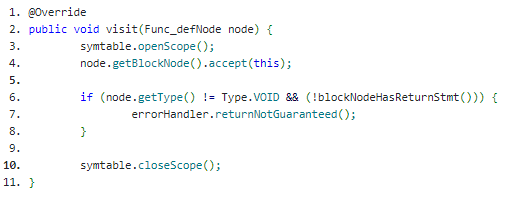
\includegraphics[scale=1.0]{figures/implementation/typeCecker/3-1-func-def-missing-return.png}}
\caption{If there is no return statement in the current scope, or an if else block where return is guaranteed throw an error.}
\label{lf05}
\end{figure}



\section{Function Structure Visitor}
The purpose of this section is to explain, how the Ezuino compiler guarantees that any function called, always has the correct structure for the given function. Before a function can be called, it must have been declared first. Except for predefined functions such as Arduino functions.
\\\\
To accomplish this goal, the Ezuino compiler implements a visitor named: “FuncStructureVisitor”. The goal for this visitor is to verify that all functions called in a given program, always has the same structure as the function declaration. This also includes predefined Arduino functions. However, since Arduino functions are predefined by the compiler, the structure of these functions are hard coded into the visitor.
\\\\
Exactly like the other visitors in the compiler the FuncStructureVisitor runs through the generated AST, starting at the first node and visiting all of its children nodes.\\
The nodes that mainly will be affected by the FuncStructureVisitor, is the nodes that has to do with functions. Specifically, these nodes are function declarations, function calls and predefined functions such as Arduino functions.
\\\\
Listing \ref{FuncDefNode} shows how a function declaration node is handled by the visitor. Since the node is a function declaration, the node must be stored in a symbol table for the current scope. this is done so that when the visitor meets the function call node, it can look up in the symbol table to find how the function was declared.\\
As seen on line 3, the function declaration is stored in the symbol table with the function id and the node.
\begin{lstlisting}[caption={Visit method for FuncDefNode in FuncStructureVisitor}, label={FuncDefNode}]
    $$@Override
    public void visit(Func_defNode node) {
        symtable.enterSymbol(node.getId(), node);
        node.getBlockNode().accept(this);
    }
\end{lstlisting}
\noindent\newline
Listing \ref{customFuncCall} shows how a custom function call is handled by the visitor. The name CustomFuncCall tells us that this is not one of the predefined functions in the compiler, but instead a function that has been declared by a user.\\
Since this is a custom function call, the compiler does not know what the structure of the function is. therefore, it must search the symbol table for a function with the same id as the call.\\
Once the correct declaration has been found, the visitor compares the parameters of the function call with the parameters of the function declaration. If these do not match, an error has occurred and is thrown to the errorHandler.\\
Similarly, if the visitor cannot find a function declaration with the same id as the function call, an error has occurred and is thrown to the errorHandler.
\begin{lstlisting}[caption={Visit method for CustomFuncCallStmtNode in FuncStructureVisitor}, label={customFuncCall}]
$$@Override
public void visit(CustomFuncCallStmtNode node) {
    Func_defNode funcdef = (Func_defNode) symtable.retrieveSymbol(node.getId());
    matchParameterList(node.getId(), node.getParameters(), funcdef.getParameters());
\end{lstlisting}
\noindent\newline
Listing \ref{matchParameterList} is the private helper method, which compares parameters of function calls. It is the same method used in line 4 of listing \ref{customFuncCall}.\\
As the function structure visitor’s job is to verify that the structure of function is correct, this private method is one of the core functions of the visitor.\\
The idea behind verifying the structure of functions is to compare the types of the parameters of the function. This involves comparing the parameters of the function call and the function declaration. For the function call to be correct, the parameters must match the parameters of the function declaration.\\
To do this, the method takes a list of function call parameters and a list of function declaration parameters as input.
\\\\
First, the method compares the number of parameters of both the call and declaration. If they are not the same, an error has occurred and is thrown to the errorHandler. This happens on line 3-5 of the listing.\\
Secondly it compares the types of the parameters, in order, of both the call and declaration. If they are not the same, an error has occurred and is thrown to the errorHandler. This happens on line 7-11 of the listing.
\begin{lstlisting}[caption={Private helper method for verifying function parameters in FuncStructureVisitor}, label={matchParameterList}]
    private void matchParameterList(String functionname, List<AExpr> callparams, List<DclNode> defparams) {
        int parametercount = callparams.size();
        if (parametercount != defparams.size()) {
            errorHandler.parameterLengthError(functionname);
            return;
        }
        for (int i = 0; i < parametercount; i++) {
            AExpr callParam = callparams.get(i);
            DclNode dclnode = defparams.get(i);
            if (callParam.getType() != dclnode.getType()) {
                errorHandler. parameterTypeError(functionname);
            }
        }
    }
\end{lstlisting}
\noindent\newline
Listing \ref{AnalogReadNode} is an example of a predefined function in the compiler and shows how the visitor generally handles predefined function calls.\\
In this case the function call is to AnalogRead, which is an Ezuino specified function. In the case of AnalogRead, it is necessary to perform an additional check for the size of the int parameter, since Arduino only handles small bit sizes. The additional check occurs on line 8. This check is not present for all predefined functions.
\\\\
Since AnalogRead is a predefined function, verifying the function structure is relatively simple. The reason for this is that because the function is predefined, the compiler already knows what parameters are required for the call. Predefined functions therefore have hard coded parameters, which cannot be changed at runtime.\\
As seen in line 3, the expected type of the AnalogRead function is an int. And since there is only one type, the function only takes one parameter.\\
Additionally, the parameter must be held within either an IntegerLiteral node or a IdNode. This is to ensure that only the correct int node is the parameter for the function call. A check for this occurs on line 5-6.\\
Lastly, a call to compare the parameters is made on line 9.
\\\\
Other predefined functions are handled similarly to the AnalogRead function. The main detail that changes is how many parameters the function has and which types the parameters have.\\
Additionally, only the Arduino functions that use small bit sized ints are required to have the int size check.
\begin{lstlisting}[caption={Visit method for AnalogReadNode in FuncStructureVisitor}, label={AnalogReadNode}]
$$@Override
public void visit(AnalogReadNode node) {
    Type[] expectedType = {Type.INT};
    AExpr firstParam = node.getParameters().get(0);
    if (!(firstParam instanceof IntegerLiteral || firstParam instanceof IdNode)) {
        errorHandler. invalidFunctionParameterError(node.getID());
    }
    checkArduinoRange(firstParam);
    checkFuncParameters(node.getID(), node.getParameters(), 1, expectedType);
}
\end{lstlisting}
\noindent\newline
Listing \ref{checkFuncParameters} shows the private helper method for comparing predefined function parameters. Similarly to the private method in listing \ref{matchParameterList}, the purpose of this function is to verify function calls and are therefore also a core part of the visitor.\\
The idea behind the checkFuncParameters method is the same as the matchParameterList. However, since this is for predefined functions, it compares function parameters with required types. For the function call to be correct, the parameters must match the predefined types.
\\\\
First, the method confirms that the amount of parameters is the same as required. If they are not the same, the function call is incorrect and an error is thrown to the errorHandler. This check occurs on line 2-3.\\
Secondly the method verifies that the parameters have the correct types in the correct order. If the types are not the same, an error is thrown to the errorHandler.\\
The comparison is done by calling another helper method, which compares two types. This check occurs on line 5-7.
\begin{lstlisting}[caption={Private helper method for verifying predefined function parameters in FuncStructureVisitor}, label={checkFuncParameters}]
private void checkFuncParameters(String nodeId, List<AExpr> parameters, int requiredParameters, Type[] typeList) {
    if (parameters.size() != requiredParameters) {
        errorHandler.parameterLengthError(nodeId);
    }
    for (int i = 0; i < requiredParameters; i++) {
        if (parameters.get(i) != null) {
            checkSpecificType(parameters.get(i), typeList[i]);
        }
    }
}
\end{lstlisting}
\noindent\newline
The five listings of code looked at in this section, should supply a general idea of the purpose of the Function Structure Visitor and how it works.\\
Not all of the visit functions were reviewed, but the few selected ones prove good examples of their implementation.
\\\\
Summing up, the idea of the visitor is to check for declared functions and store them. Then when a function call occurs, check which type of function has been called.\\
For custom functions calls, the visitor searches for a function declaration with the same Id as the call. If such a declaration exists, it compares the parameters of the call with the declaration.\\
For predefined function calls, the compiler already knows which type of parameters are required and can therefore perform its parameter check, without searching for a function declaration.
\section{Parse Tree}
By passing the grammar file with the EBNF (Listing \ref{code:ebnf}), ANTLR generates both a lexer and a parser. The generated lexer and parser is ready to read and recognize any text passed to it. From the parser the group now has the ability to program any further usage of the recognized language.
\\
However, ANTLR4 generates a parse tree (also known as Concrete Syntax Tree) which is the literal recognition of token in the programming language. Each and every symbol is included in this parse tree, including terminal symbols like equality signs (\texttt{:=}), parenthesis(\texttt{()}) and keywords (\texttt{if}). These are named after the terminals and non-terminals in the EBNF file. While one could potentially work with these tokens directly, it's hard to navigate with all the extra tokens on the nodes.
\\
As an implementation, all the nodes in the parse tree were converted into an abstract syntax tree nodes. This is done by using a class called \texttt{BuildAstVisitor} which is a subclass of the \texttt{BaseVisitor} provided by ANTLR. In actuality, this provides a visitor pattern to traverse through the parse tree. During the traversal, the individual nodes in the AST are created from the information available information.
Seen in \ref{code:visitFuncDef} is a snippet where an AST node is created. The \texttt{Func\_defContext} has access to both the rules and the actual text that was parsed. In this case, it is the syntax
\texttt{func int test() \{\}}. While the syntax is pretty short, the word \texttt{func} is not essential for further processing in the AST. This is contained within the node itself (since it is a \texttt{Func\_defNode}) and is such not used. Something special in this case is also the fact that special functions \texttt{Setup} and \texttt{Loop} nodes are detected. This makes it easier to distuingish which node is being processed in further processing of the AST.
\\
\begin{lstlisting}[caption={Visit method for \texttt{Func\_defContext} in \texttt{AstBuildVisitor}}, label={code:visitFuncDef}]
$$@Override
public AstNode visitFunc_def(EzuinoParser.Func_defContext ctx) {
    String ID = ctx.ID().getText();
    Type type = getType(ctx.type());
    List<DclNode> parameters = new ArrayList<DclNode>();
    BlockNode blockNode = (BlockNode) ctx.block().accept(this);
    for (DclContext child : ctx.parameters().dcl()) {
        parameters.add((DclNode) child.accept(this));
    }
    switch(ID) {
        case "Setup" : return new SetupNode(ID, type, parameters, blockNode);
        case "Loop" : return new LoopNode(ID, type, parameters, blockNode);
        default: return new Func_defNode(ID, type, parameters, blockNode);
    }
}
\end{lstlisting}
\section{Symbol table visitor}
\ref{Block_Structure_Symbol_Tables}
The symbol table is a data structure that enables storage of variables across different scopes. It is used whenever during the visitor pattern there is a need to reference another node in the abstract syntax tree. This could, for instance be whenever a variable is used within a scope. To find out the type of the variable, there is a need for a data structure which can search up though the different scopes of the program (E.g. from local to function to global scope).
There are multiple ways of implementing it and storing the data in memory for further investigation, but the Ezuino compiler only has references in each visitor to the symbol table.
The data structure is a stack and the elements in the stack are called \texttt{SymbolTable}. Each symbol table is a simple hash map with a reference to the parent level in the stack. By holding the reference to the scope above, it is possible to make a recursive search algorithm when looking for the variable in different scopes.
The data structure that contains the stack is called \texttt{SymbolTableHandler} and provides an API for storing and retrieving references to other nodes in the abstract syntax tree. By implementing it this way, the storage and searching is hidden for potential visitors which needs to store variables.
During the compilation, there are 4 visitors that use the \texttt{SymbolTableHandler}.
\begin{enumerate}
    \item \texttt{SymbolTableVisitor}: Stores function and variable declarations to check if there is declaration before use of functions and variables
    \item \texttt{FuncStructureVisitor} Stores functions to check if the function calls invoke with the correct parameters
    \item \texttt{MissingReturnStmtVisitor}: Stores return node to check if the function has a return statement if the returntype is a type.
    \item \texttt{ReturnStmtTypeCheckVisitor}: Stores function declarations to check whether the type of the return statement is the same as the function is declared to return
\end{enumerate}
\section{Code Generation}
Nearing the end of the compiler run, after having done all the contextual analysis described in the different visitor sections, you end up with a Decorated Syntax Tree (DST).\\
This tree has been decorated by all of the visitors previously described and therefore lives up to all rules of the programming language. This means that the DST contains all of the data, the other visitors has decorated the tree with. Because of this, we can now use the DST to generate code.\\
The purpose of this section, is to describe how the Eziuno compiler, uses the DST decorated by all other visitors, to generate code.
\\\\
There can be multiple code generators, as they follow the visitor pattern to generate the code. This is the point where the designer of the compiler decides what target language(s) the compiler should have.

\subsection{Target languages}\label{CodeGen:TargetLanguage}
There are several different target languages that would be wise to compile to. These could be C, Assembly or Java-bytecode. Considering that our language is intended for home automation purposes, compiling to C isn't a bad idea, as it makes it easier for us to optimize the compiler to be memory or speed effective.\\
Furthermore, the gcc compiler is on many platforms and architectures, making it trivial for us to port it from one platform to another. Java bytecode is also a good option for a target language, as it runs on the JVM, which is implemented on many platforms too, though it should be noted, that java bytecode still works with a class-based structure, meaning we would have to model our imperative language in an object-oriented space.
\\\\
Compiling to an intermediate language is usually a decent idea, as it lets our own language build on top of an already existing compiler-collection, to allow our code to run on many platforms out of the box.\\
Considering that the alternative is to compile to a platform-specific assembly language and that there are better options for us to compile to, we will therefore not be making a platform-specific compiler.
\\\\
A good approach for high level languages is to translate to a intermediate low level language, that already have implementations for most hardware.\\
Implementing a language this way, means that you can implement a code generator for the high level language to target language, which then can be use to generate code for other languages.\\
Doing it this way, means that instead of making a high-level $*$ low-level number of compilers, you only have to make a high-level $+$ low-level number of compilers.\\
This does add abstraction, but might also add complexity if either the source language or the destination language, implements structures that are hard or impossible to implement.\\
Examples of compilers with intermediate languages are Java and C\#. Java compiles Java Bytecode which is the instruction set of the Java Virtual Machine. C\# compiles to Common Intermediate Language, which is then run on the Common Language Runtime.

\subsection{Code generator visitors}
The Ezuino compiler implements three different code generator visitors, each their own target language. The three visitors are C code generator, Arduino code generator and lastly Java Bytecode code generator. The code generators will be discussed in this section, in the same order they were mentioned.
\\\\
As mentioned section \ref{CodeGen:TargetLanguage}, there are many options for different target languages for a compiler. For Ezuino, three targets have been chosen: Standard C, Arduino and Java Bytecode.\\
Since the goal of the project is to compile to Arduino, one might be confused as to why the Ezuino compiler also implements a C code generator. The C code generator was the first code generator to be implemented in the Ezuino compiler. It was used as an proof of concept code generator and was mainly used to easily verify and compile test programs, to a non-Arduino language platform.\\
Because Arduino is a language very similar to C, C was a perfect language to implement the first proof of concept code generator.\\
After the C code generator was fully implemented, because Arduino is so similar to C, the Arduino code generator was practically extended from the C code generator. Only minor changes to the original C code generator was necessary to convert the C code generation into Arduino code.\\
Additionally, the Arduino code generator implements code generation for special Arduino functions. these are only a part of the Arduino code generator, not any of the other code generators.
\\\\
%Next the Arduino code generator...
Because that the C code generator is so similar to the Arduino code generator, both of these will be discussed together.\\
The code generators all uses a Java StringBuilder to build up, what will eventually become the final program in the target language. Using the visitor pattern, the code generators visits each node in the DST and appends the necessary code to the StringBuilder. The code appended to the StringBuilder depends on which node is visited, when walking the DST.\\
The first code snippet is from the C code generator. This snippet shows how the necessary C headers are appended to the StringBuilder (listing \ref{io01}).\\
\begin{lstlisting}[caption={Visit start node in C code generator}, label={io01}]
$$@Override
public void visit(StartNode node) {
    // includes
    builder.append("#include <stdio.h>\n" +
        "#include <string.h>\n");
    // start tree search
    node.getDcls().accept(this);
    node.getStmts().accept(this);
    // prints the final string
    out.print(builder.toString());
}
\end{lstlisting}
\noindent\newline
The second code snippet is from the Arduino code generator. This shows two visit methods for special Arduino functions, in the Arduino code generator. The first is a method for generating a \texttt{Delay} method from Arduino. The second in a method for generating a \texttt{DigitalRead} method (listing \ref{io02}).
\begin{lstlisting}[caption={Visit delay node and digital read node in Arduino code generator}, label={io02}]
$$@Override
public void visit(DelayNode node) {
    builder.append("delay(");
    node.getParameters().get(0).accept(this);
    builder.append(");\n");
}

$$@Override
public void visit(DigitalReadNode node) {
    builder.append("digitalRead(");
    node.getParameters().get(0).accept(this);
    builder.append(")");
}
\end{lstlisting}
\noindent\newline
The last visitor is the Jasmin code generator.\\
Unlike the previous two visitors, the jasmin code generator doesn't compile to a C-like language, but rather to Jasmin, which is an assembler-representation of Java bytecode. This is quite different from parsing to C or Java, as the scoping rules are a bit different, either being completely flat inside a given function, or more of a nested structure if one is using classes and access modifiers.\\
This combined with a register-based storage model means, that the compiler has to manually keep track of the allocated registers, and when it is safe to overwrite a given register with another value. This is currently handled when the Jasmin visitor visits a block node in the AST.\\
The code snippet in question can be seen in listing \ref{code:JasminBlock}. Note that a copy of the variable environment is reset to its pre-block state after the entire block has been generated. This is so that a variable declared in an inner scope will take precedence when being referenced in an expression, compared to a variable of the same name declared previously in an outer scope, while still "deallocating" the inner variables after the block has been processed.
\begin{lstlisting}[caption={Code for visiting a block in the JasminCodeGeneratorVisitor}, label={code:JasminBlock}]
$$@Override
public void visit(BlockNode node) {
    List<String> oldVariableEnvironment = new ArrayList<String>(currentVariableEnvironment);
    List<String> oldLocalFunctions = new ArrayList<String>(currentLocalFunctions);
    // < Code for visiting children omitted for readability>
    currentVariableEnvironment = oldVariableEnvironment;
    currentLocalFunctions = oldLocalFunctions;
}
\end{lstlisting}
\\\\
Furthermore, it should be considered that the JVM is a stack machine, and thus it should be taken into consideration, when writing code for it. Though this is mostly a fact to be considered when evaluating expressions, though it is also important when it comes to function calls (or method invocations, as they are parsed down to), as these use the top i elements of the stack as parameters, and then push the return value of the function back on the stack.\\
The stack also plays a role in some of the more complex implementations (namely prints and strings), as these use object references like in Java, but on the stack, like any other value. It isn't terribly hard to write the (java) method invocations, but you do have to keep your wits about you, as the order of the stack matters, and the typing syntax of the JVM gets a bit longer and incomprehensible, when referencing custom types like "String".
\\\\
%Conclusion/ending? Byte code: implementing arduino functions, so that we can transform byte code into arduino
\section{Error Handling}
\label{error-handling-chap}
Error Handling is a vital general tool, which is used for the users to get an overview of the errors, which they made during their time coding the Ezuino programming language. The error handling tool is a part of the ANTLR V4 Runtime library, which uses its error handler as an interface which deal with syntax errors, which get encountered during the parsing of the ANTLR generated parse files. \\
\\
First, we use the ANTLRErrorListener class, which is an interface implementing methods for the different errors, the user may make during the program. The listener can report anything from syntax errors to ambiguity reports.
\begin{lstlisting}[caption={Start of the ErrorListener class}, label={eh01}]
private int errorCount;
private ErrorHandler errorHandler;

public ErrorListener(ErrorHandler errorHandler) {
    this.errorHandler = errorHandler;
    this.errorCount = 0;
}

$$@Override
public void syntaxError(Recognizer<?, ?> recognizer, Object offendingSymbol, int line, int charPositionInLine,
    String msg, RecognitionException e) {
    this.errorCount++;
    errorHandler.syntaxError(errorCount, msg, line, charPositionInLine);
}
\end{lstlisting}
\noindent\newline
The one we’re interested in is shown in listing \ref{eh01}. In this code, we’re inside the ErrorListener class, which implements the ANTLRErrorListener interface.  In listing \ref{eh01}, we got two global variables, errorCount, which is used to count the number of errors, ANTLR found during the parsing. The ErrorHandler instantiation is from the ErrorHandler class, which handles a specific type of errors during the AST, and covers more abstract error handling, for example, cast exceptions, type exceptions and many more. The ErrorHandler class will be described later in this section. \\
\\
The only method we are interested in is the syntaxError method, which is recognizing syntax errors made by the users. As an example, if the users input the code (int int), this would be a violation of the ANTLR grammar, as it’s two literals, the scanner review as int type declarations, without any ID after both the declarations. If the scanner recognizes this error, it will not run the visitors, or future visitors through, as the error was caught in the earlier stages of the process.
\begin{lstlisting}[caption={Start of main}, label={eh02}]
CharStream cs = CharStreams.fromFileName("src/main/code.ezuino");

ErrorHandler errorHandler = new ErrorHandler();
AstNode ast = syntaxAnalysis(cs, errorHandler);
if (errorHandler.hasErrors()) {
    errorHandler.printErrors("Syntax errors");
    return;
}
\end{lstlisting}
\noindent\newline
Listing \ref{eh02}, is from the Main class in the Ezuino program. This class executes all the lexers, parsers, visitors, error handlers in order, to provide flow in the compile process. In listing \ref{eh02} on line 1, we use a character stream to read the written Ezuino program file from the code.ezuino file. We then create a new error handler, which we use the syntax analysis method to go through the parser and lexer file generated by ANTLR from the Ezuino grammar file. \\
\\
Going back to the ErrorHandler class, we got 3 methods, which has the main functionality of the error handler. 
\begin{lstlisting}[caption={Start of ErrorHandler class}, label={eh03}]
private List<ErrorMessage> messageList = new ArrayList<>();
private int errorCount = 0;

public boolean hasErrors() {
    return errorCount != 0;
}

public void printErrors(String reason) {
    if (hasErrors()) {
        StringBuilder sb = new StringBuilder();
        String errmsg = "##  " + reason + "\n -- ## ERROR OUTPUT CONSOLE ## -- ";
        sb.append(errmsg + "\n");
        for (ErrorMessage message : messageList) {
            sb.append(message + "\n");
        }
        System.err.println(sb.toString());
    }
}
\end{lstlisting}
\noindent\newline
Listing \ref{eh03}, is a snippet from the ErrorHandler class. On line 1, we got a List, which contains all the error messages found during the contextual analysis, reported by errors in the AST visitor classes. The method hasErrors() from line 4, checks if the errorCount on line 2, is bigger than 0. If it is, that means that the error handler has added an error to the error list.\\
Finally, from line 13 we got the printErrors() method, which prints the methods, which is in listing \ref{eh04}. First, it checks whenever there are errors, then it prints all the messages in the List, by running a for each loop for 18. 
\begin{lstlisting}[caption={three different error messages from the ErrorHandler class}, label={eh04}]
public void varAlreadyDeclared(String character) {
    addError(new SyntaxError(ErrorType.ERROR, "Variable " + character + " is already defined in this scope."));
}
public void funcAlreadyDeclared(String character) {
    addError(new SyntaxError(ErrorType.ERROR, "Function " + character + " is already defined in this scope."));
}
public void unexpectedType(ITypeNode node, Type type) {
    addError(new GeneralError(ErrorType.ERROR, "Unexpeced type! Expected: " + type.name() + ", was " + node.getType().name() + " - Node: " + node));
}
\end{lstlisting}
\noindent\newline
Listing \ref{eh04} has 3 methods, which is being used within the visitors. The methods take either string as ID’s, or nodes and do in-method conversions of messages, which are being added to the List on listing \ref{eh03}, line 1. The SyntaxError and GeneralError classes both contain different string representations of each error. 
\begin{lstlisting}[caption={The syntaxError class}, label={eh05}]
public class SyntaxError extends ErrorMessage{

    public SyntaxError(ErrorType errorType , String errorMessage) {
        super(errorType, errorMessage);
    }

    $$@Override
    public String toString() {
        return String.format("SYNTAX %s %s", this.getTypeString().toUpperCase(), this.getErrorDescription());
    }
}
\end{lstlisting}
\noindent\newline
Listing \ref{eh05} is an example of the SyntaxError class, for every error method in Listing \ref{eh04}, which constructs a new SyntaxError, will need the input of an Error Type and Error Message. Then, the toString() method from line 8, returns a string with a specific format, for this syntax error. 
To get an overview of these classes together, a relationship diagram has been created and can be reviewed in figure \ref{eh06} below.
\begin{figure}[H]
\centering
\frame{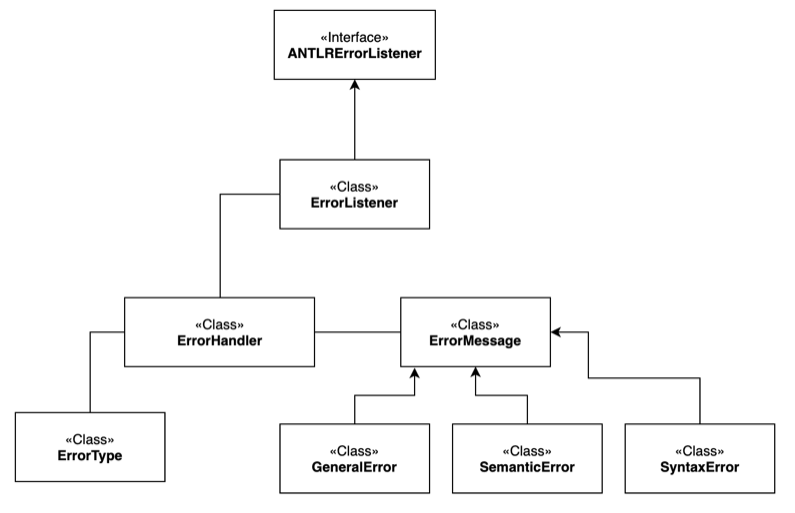
\includegraphics[scale=0.45]{figures/implementation/eh06.png}}
\caption{Class diagram of the error classes}
\label{eh06}
\end{figure}

\chapter{Test}
In this chapter, we go through the tests, which got made during the development of the Ezuino programming language. At the beginning of the project, the only tests which could be done were using the language made by the ANTLR grammar file and testing different dummy programs, and test whenever ANLTR report any ambiguity or syntax error within the code entered. Multiple programs got written, to ensure that we got around every syntax and scenario possible, to avoid any future error, once we’ve started building the Concrete Syntax Tree (CST) and the Abstract Syntax Tree (AST).  One of the programs can be reviewed in listing \ref{ex02}.
\\\\
\section{JUnit Testing}
Once the development of the compiler in Java has started, JUnit testing has been used during the remaining process. This section will go through some of the JUnit test, which has been written during the development process. The tests have been categorized into three sections, the tests for the concrete syntax tree, the abstract syntax tree and the lexer and the parser CST, AST, and Lexer/Parser test.
Starting from the beginning of development, we look at some of the Lexer and Parser tests, which is the classes ANTLR 4 has generated and using the ANTLR maven package, can use. In these test classes, we use the Error Handler, which was explained in \ref{error-handling-chap}, to check whenever there is an error, during the lexing/parsing of a small code snippet. If the error handler finds an error, depending on the assert, the test will either fail or pass.\\
Listing \ref{test1} shows a method, which is used to initialize the error handler, lexer and parser with the code, as inputted by a string.
\begin{lstlisting}[caption={Private function to run a test program}, label={test1}]
private ErrorHandler parseProgram(String program) throws IOException {
    CharStream stream = CharStreams.fromString(program);

    ErrorHandler errorHandler = new ErrorHandler();
    ErrorListener el = new ErrorListener(errorHandler);

    EzuinoLexer lexer = new EzuinoLexer(stream);
    CommonTokenStream tokens = new CommonTokenStream(lexer);
    EzuinoParser parser = new EzuinoParser(tokens);

    lexer.removeErrorListeners();
    lexer.addErrorListener(el);
    parser.removeErrorListeners();
    parser.addErrorListener(el);
    parser.start();

    return errorHandler;
}
\end{lstlisting}
\noindent\newline

On listing \ref{test2}, we have the first test, which a simple integer declaration, where we declare the variable a. We assert that the errorHandler should not have any errors, as this is the correct syntax in this case – using the hasErrors() method, which is a part of the error handler class, and will return an Boolean value.
\begin{lstlisting}[caption={Simple declaration test}, label={test2}]
$$@Test
public void testDcl() throws IOException {
    ErrorHandler errorHandler = parseProgram("int a");
    assertFalse(errorHandler.hasErrors());
}
\end{lstlisting}
\noindent\newline

Listing \ref{test3} shows the test of the expression (1 * 10), where we test if both the right and left side nodes of the MultiplicativeExprNode are of type Integers. If they aren’t, we can already throw an exception. Next, we’re checking if the values of the left and right nodes are the ones that we’ve entered in our expression. In this case, we assert that the left node has the value of 1, and the right node has the value of 10. We also check that the operator in this expression is a multiplicative operator.\\
The code generation tests for Java bytecode and C, has been tested by taking the Ezuino program, and comparing it to an expected output of the C programming language. If the output is correct, the tests are successful.
\begin{lstlisting}[caption={Simple multiplication expression test}, label={test3}]
$$@Test
public void simpleMultiplicativeExprTest() throws IOException {
    EzuinoParser ep = createParser("1 * 10");
    MultiplicativeExprNode topNode = (MultiplicativeExprNode) ep.expr().accept(visitor);

    assertTrue(topNode.getLeftNode() instanceof IntegerLiteral);
    assertTrue(topNode.getRightNode() instanceof IntegerLiteral);
    assertEquals("1", ((IntegerLiteral)topNode.getLeftNode()).getVal());
    assertEquals("10", ((IntegerLiteral)topNode.getRightNode()).getVal());
    assertEquals("*", topNode.getOperator());
}
\end{lstlisting}
\noindent\newline

\section{Continuous Integration}
During the development of the programming language, more tests has been added in the development process. The final number of tests, is around 500, in multiple classes. This is a significant number of tests to run each time an AST or node has been changed, so Continuous Integration (CI), has been deployed, to automate each test and compile the software after each Git Commit (GC) or Pull Request (PR).  The CI used for this purpose was Travis CI, which is a free CI service for public git repositories. \\
\begin{figure}[H]
\centering
\frame{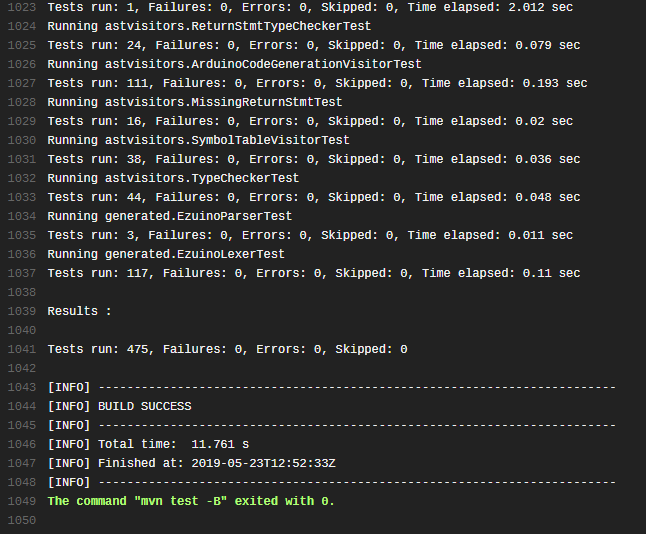
\includegraphics[scale=0.8]{figures/newfuk.png}}
\caption{Screenshot from TravisCI website for Ezuino project}
\label{testa}
\end{figure}
On figure \ref{testa}, a Travis build has run on a GC, which has recently been committed. In this result, we can see that the 475 tests have been run successfully, and the program ran without any error. If any of the tests or main could not run, Travis would have thrown an error. \\
\\
This chapter has been going through a few of the around 500 tests made in this project and given an insight in the tests process which has been made during the development of the Ezuino programming language. It is very essential to avoid errors in the compiler in a programming language, so testing of features has been prioritized, however, there are still testing forms like code coverage and whitebox (branch testing), which has not been done at this time. If the Ezuino programming language were to get a commercial release, these tests are essential to provide a large sum of error or failure correction, as a programming language is very abstract.
\section{User Test}
In this chapter we present the feedback we were given from on Ezuino. The test person was a student in psychology second semester having never programmed before but interested in participating in the test. The test was conducted by giving the test person a guide that both covered basic programming terms, the syntax of Ezuino with code examples and a set of assignments. The guide can be seen in appendix \ref{user_guide_appendix}. The test person was taking the test together with a test moderator, in order to ensure the participant did not get completely stuck at an task either due to being completely new to programming or due to the guide being unclear. After the test the participant was asked give feedback on the programming language and to review key points about Ezuino where it differed from C. The screen and communication during the test was recorded for intern review with consent.
We got the following feedback
\begin{itemize}
    \item "AND" and "OR" was preferable to  $\&\&$ and $\|\|$ and boolean was prefered to 0 and 1. 
    \item The data types could be less technical named so it is easier to understand without a background. An example from the test person was that string could be called "words". We asked if "text" would also be easy to understand as we felt it was more precise for more use cases of strings, and the test person said it was just as good. It could be observed from the test person that they fairly fast forgot was the meaning of int, double and boolean was after having read the explanation. While this could simple be due to having to comprehend many programming terms in a short time span, it could also be due to the name of the data types being less intuitive, making them harder to remember the meaning of.
    \item Strong typing also came as a surprise to the test person. That 32 gave an type error when assigned to double was an example of this.
    \item We showed the test person the list we had intended to implement as versions of arrays that did not need malloc and free and functioned like ArrayList in Java but without being object oriented. The test person did prefer it, but also suggested a method to find the index of a value in a string list in case they had a hard time keeping track of what index each value was saved. Interestingly enough the index of an value is often easier to remember in arrays compared to list when looking at source code, since you have use the array index when you assign entries in an array. This suggest that having both arrays and a structure similar to list would be good since they both have different advantages for people new to programming. In both arrays and list the test person would prefer that entries in the array would start from index 1 instead of 0.
    %\item To our surprise the test person did not dislike the idea of ending statements with ";" like in C, comparing it to dot in a sentence. According to the test person dot could even substitute ";". In the same manner of thought the test person also suggested that the starting letter of keywords that can start a line could also start with uppercase, making it more like an sentence.
    \item According to the test person ":=" and "=" made sense compared to C, ":=" reminding the test person of assignment in a math program previously used in her study.
    \item During the test there were a few times the test person forgot declaration before assignment. This could be interpreted as declaration before usage being unintuitive to new programmers. 
\end{itemize}

Besides those points the test person also gave some feedback on our current error messages, making us aware that both the error messages from type mismatch and syntax error had some room for improvement.









%This guide can be seen in appendix (SKRIV APPENDIX IND).  
%The test setup is simple. A table, with a chair together with a computer running a text editor with one text file “code.ezuino”, and running the programming language in the background. After the compiler has compiled the program, the output program was then copied into an Arduino IDE, and executed on the Arduino. The test person was handed a syntax specification table, which contain a small explanation of what each operator did, and we tried to give them two simple tasks, which they will use the language, only using the syntax specification table. \\
%\\
%The first test which got presented to the test person were a simple programming task, where they had to construct a “hello world” string in a function, which is outside the setup and loop function, and run it the function once. At first, the test person was confused, however, after presenting them to how the setup and loop functions works, and told them what each of them did, they replicated a function, similar to the setup function, and insert a print statement, which printed “hello world”. The test person had an issue understanding functions, as they wanted to run the program right after they have added their new function. When a dialog with the test person, on how functions work, and that the code only executes the setup and main, and you must call the function in each, the test person completed this task.\\
%\\
%The second test which got presented to the test person, were harder task, but builds on the previous task, and provides a code example written C, with Arduino libraries attached. The tasks were to learn about the user’s interaction between the Arduino and applying code to get a result. The programming was to get data from a temperature sensor and get the temperature out in the Arduino console. By already providing the body, with setup, loop and serial begin as the first test setup, the only explanation we gave the test person beforehand, was that floats form the program example was double in our language, and that they had the same functionality. As the Ezuino programming language already had a lot of the library features which Arduino reside, the user could replicate the code into the Ezuino programming language, with one missing component, the language was missing (println – prints on a new line). We asked the test person whenever he understood the difference between the normal print and the print new line method, and he answered yes, and concluded that it could be a good feature to include.\\
%\\
%We can conclude from this limited test that language specification and documentation are everything. Good explanations of where to start, what each do, and where to use each feature where is vital, and can get people, with no programming experience to produce functional code. In goal with this project, is to avoid having a teacher, sitting next to the person programming, but to learn it from a set of instruction and specification. The test setup with the temperature sensor used for the second test was not user friendly for users who do not have experience at all. If home automation for Arduino would ship, we should provide easy and ready packages, where the user only should plug the Arduino into their computer and execute the code. At last, there was a feature which we did not think should have been added. The println feature was understood by the user, and as it can provide a good functionality to the program, we added this feature in the language.
%\\

\chapter{Discussion}
In this chapter, we will discuss the aspects of the development of the Ezuino programming language. We will review the intended goal of the programming language and reflect whenever the final product reflects the goals, which were set for the programming language in the beginning.   
\\\\
In the problem definition, the following got defined:  
\\\\
\textit{In a world of increasing microchip automation, programming becomes a basic mainstream skill. To assess this, a programming language should be designed, which can be used for people, with little or no prior programming knowledge. } 
\\\\
The problem definition leans closely towards that the final programming language should be easily used for new or beginners. The syntax was designed within the language design criteria to be readable, writable and reliable. Using these criteria, we were able to choose a minimal syntax, allowing for the core functionality for an Arduino. Before starting to write the syntax, we are looking at the core programming language an Arduino is running, C with Arduino libraries. We then took the main features from the C programming language and found multiple alternatives of which syntax is best for each feature. We decided to keep the language very minimal, so most datatypes and control flow functionality is limited to the users being able to learn it fast, and don’t get overwhelmed by the features available. In the beginning, we had a general idea of how the program syntax should look like, from when we as developers started to program. After setting up this syntax, we had a user test with a third-party test person, who fitted the end goal group well, as they did not have any previous programming experience. The feedback received by this was surprising well for most of the syntax, other than naming some of the attributes and strong typing. The test person managed to create a small program, using the help sheet provided, which is a very good early reflection towards the program definition, where it should be used or learned by the target group.  
\\\\
During the development of the Ezuino programming language, reserved keywords was a greater challenge as well. The Java programming language, which is the language the programming language got developed in, had a lot of reserved keywords, which must be handled in the grammar files, and as well inside the compiler as well. As the end goal was towards the Arduino, which is using a library for most of its special syntax, the Ezuino programming language should know about these “special syntax” as well. Arduino uses the C programming language, with a special library designed to make development and usage of the Arduino easier for the users. This library was large, and most of the library content wouldn't fit the description of the problem definition, where the language must be easy to use and learn. It was decided that some of the features, which is vital for the Arduino to run, and the features with the core functionality and makes the most sense for the users, got added as well. In this consideration, we had to reflect whenever the input of the function like pinMode, which in the Arduino specification accepts both the HIGH / LOW keywords and using numbers which HIGH and LOW are defined in the library as 0 and 1. The Booleans in the Ezuino language is already defined as true and false, where the 0 and 1 are hidden for the user, so the same should be considered here, where we force the user to use the HIGH / LOW syntax for these special functions. \\\\
Scopes in the Ezuino programming language was thought to be the same, as in the C programming language, as this is the core language used for the Arduino. The reason for this, is that that the user in the user test could understand how it works, and it builds a form of hierarchy on each scope, meaning that you can access what has been added on a higher level, but not in the future and not in closed scoping. (MB BS???)  
\\\\
In the Ezuino programming language, it is vital to declare a variable before doing statements. This has been ruled in the ANTLR grammar file. The idea behind this, is to “create a contract” with the users, that they must do it consistently, both for the readability, but also to keep track of where and what variables have been declared where. There has been a lot of discussions whenever it is good to force the users to write more lines of syntax than necessary, however, it may be changed in the future if more user feedback can be assessed, even though new users most likely would find it normal, as it is most likely their first programming language that they have used.  
\\\\
Missing: types and tests, then done 


\chapter{Future Scope of the Project}
If given more time to work on the project it would make sense to improve several aspects of Ezuino. There were both feedback from the user we could account for and some features we think might make sense to extend the language with in the future.
The feedback from the user suggested we should change our data type syntax and shift to weak typing. Data type names like text and float instead of string and double are more common terms for the data types that people without programming experience are more likely to understand. Weak typing also increases writability by making the language less strict, better accommodating people less experienced in using types in practice. Although this might lead to less reliability code due to using implicit casting without intending to. \\
We also got feedback on the dynamic array implementation called list we had intended to include in the language but had to conclude was out of scope due to our time limit. If given the time the data type should be implemented as it not only serves the purpose of arrays in Arduino C which is essential for many programming applications but also are a easy way to implement dynamic arrays. This data type would presumably have increased writability as dynamic arrays are fairly complex to implement in Arduino. This might also have increased writability due to new programmers more often opting to use dynamic arrays when it fits the situation more when a more high level data type is available. \\
Besides those 



, being easier to was preferable as an additional option to arrays.

using the feedback from the user test; better type names, weak typing at least so int can be written in double types
dynamic arrays or as we called them list
\\\\
things we didnt generally have time for:

string concatenation in the Arduiono C code generator
records / structs are very useful for various tasks in arduino. For example to define data types related to whether when working with whether
parsing library. So string for example can be parsed to other data types.


In this project, the compiler does not directly interact with an Arduino or Arduino IDE. The compiler code generates the input code written in the Ezuino programming language, and output multiple, which one being Arduino C. This Arduino C generated code can then be pasted in to an IDE connected to the Arduino and be run. In future developments, there could have been multiple approaches to the connectivity between the compiler and an Arduino. One way is to use a native implementation, which uses serial and parallel communication between a C compiler and the micro-controller on the Arduino. There are different AVR libraries which can compile C code and upload it to the Arduino and other microchips. It is also possible to use embedded java environment to use Jasmin java binary classes to compile with HaikuVM, which provides a solution to bring a micro-version of the JVM to the Arduino.
The options are unlimited when getting the code executed on the Arduino. This subject is to be researched further; we must assess if we need a custom coding environment.
\chapter{Conclusion}\label{ch:conclusion}
In case you have questions, comments, suggestions or have found a bug, please do not hesitate to contact me. You can find my contact details below.
  \begin{center}
    Jesper Kjær Nielsen\\
    \href{mailto: jkn@es.aau.dk}{jkn@es.aau.dk}\\
    \href{http://kom.aau.dk/~jkn}{http://kom.aau.dk/\textasciitilde jkn}\\
    Fredrik Bajers Vej 7\\
    9220 Aalborg Ø
  \end{center}


\printbibliography[heading=bibintoc]

\label{bib:mybiblio}
\appendix
\chapter{Appendix A User guide for language test of Ezuino}\label{ch:appAlabel}
\label{user_guide_appendix}

\textbf{Test assignments}
\begin{enumerate}
    \item make two assignments, one of them must be boolean
    \item make a while loop with AND and OR and equal logical statements. 
    \item Make a while loop with a boolean variable as expression.
    \item define a function and call a function
    \item make a void function with and without return
    \item make a if else in a if else.
\end{enumerate}
\begin{flushleft}
\textbf{How to start a program} 
\end{flushleft}
Every program must have a setup declared and is recommended to have a loop function declared. \\
func Setup()\{\\ 
\hspace*{1cm} statements\\
\}\\
func Loop()\{\\
\hspace*{1cm} statements\\
\}\\\\
outside of loop and setup function definitions are made
\begin{flushleft}
\textbf{1.}\\
\textbf{Variable declarations and assignment:}
\end{flushleft}
A variable is a value that is saved with another name.\\
When you first tell that an value exist it must be "declared" so it later can  get an value, which is called a assignment.\\
The right side of an assignment can be a expression or a function call.
Example:\\
int someNumber \hspace*{22mm}             \#declaration\\
someNumber := 1 \hspace*{20mm}            \#assignment\\
sumeNumber := 2/2 \hspace*{16mm}          \#expression\\
someNumber := returnTwo() \hspace*{2mm}  \#function call
\begin{flushleft}
\textbf{Statements:}
\end{flushleft}
  \hspace*{3mm} variable assignments\\
  \hspace*{3mm} function calls\\
  \hspace*{3mm} while loops\\
  \hspace*{3mm} if else statements\\
\textbf{code:} all text that is programmed is called code.\\
\begin{flushleft}
\textbf{A value can be a:}\\
\end{flushleft}
int (which is whole a number ex. 1)\\
double (which is a floating point number ex. 1.1)\\
string (text: "hello")\\
boolean (data type for logic, it has the values true and false and can handle expressions that compare to each other.\\
\hspace*{13mm} Example. \\
\hspace*{13mm} a:= true\\ 
\hspace*{13mm} a:= false\\
\hspace*{13mm} a:= 1<2\\
)
\begin{flushleft}
\textbf{2.}\\
\textbf{While loop:}
\end{flushleft}
A while loop repeats the code inside it until the condition no longer is met.\\
Example:\\
int a\\
a := 0\\
while(a<3) \{\\
\hspace*{2mm} a = a - 1\\
\}	
\begin{flushleft}
\textbf{3.}\\
\textbf{AND OR EQUAL:}
\end{flushleft}
AND, OR  and equal “written =” are used for logic
both arguments have to be true for an and statement to be true.
Example.\\
1<2 AND 2<3\\
One of them must be true for OR\\
Example.\\
1<2 OR 2<1\\
And equal returns true if the two compared values are the same.\\
Example.\\
1 = 1\\
Example with a variable:\\
int a\\
int b\\
boolean c\\
a:= 1\\
b:=1\\
d := 2\\
c :=  a = b (evaluates to c := true)\\
c := 2 = 2 AND 1 = 1   (will be true)\\
c := 2 = 2 OR 2 = 1    (will be true)
\begin{flushleft}
\textbf{4.}\\
\textbf{Function definition and function call:}
\end{flushleft}
  A function executes the code inside {} brackets when called.\\
  A function can have a type. If it have a type it must return a value.\\
  Example:
 \begin{flushleft}
 \textbf{Function definition with type:}
 \end{flushleft}
func int returnANumber()\{\\
\hspace*{12mm}	return 1\\
\}

\begin{flushleft}
\textbf{Function call:}
\end{flushleft}
Runs the statements inside the function definition and might return a value.\\
helloWorld()\\
returnOne() \hspace*{15mm} \#might return the value 1 depending on the code inside it.\\
Example:\\
int a\\
a := returnOne()
\begin{flushleft}
\textbf{5.}\\
\textbf{Function definition without type (also called void):}
\end{flushleft}
func helloWorld()\{\\
\hspace*{12mm}string hello := "hello world"\\
\}\\
If you want to end a function before it has run all code it can use return without a value.\\
Example. \\
func int returnANumber()\{\\
\hspace*{13mm} if(error)\{\\
\hspace*{27mm} return\\
\}\\
\hspace*{13mm} int a\\
\hspace*{13mm} a:= 5 + 13\\
\hspace*{13mm} return a\\
\}\\
(stops after repeating 3 times since a = 0)
\begin{flushleft}
\textbf{6.}\\
\textbf{If else statements:}
\end{flushleft}
If decides if some code will be reaches if what inside them is true. If it is not true else will be executed instead.\\
For example where the if statement is true and else will not be reached.\\ 
if(1<2)\{\\
\hspace*{11mm} int a\\
\hspace*{11mm}	a := 5\\
\} else\{\\
\hspace*{11mm} int a\\
\hspace*{11mm} a := 1\\
\}

\end{document}